\documentclass[12pt,a4paper]{article}

% ---------- Codifica e lingua ----------
\usepackage{cmap}        % Rende il PDF ricercabile e il testo selezionabile
\usepackage[T1]{fontenc} % Codifica corretta (essenziale per l'italiano e gli accenti)
\usepackage[utf8]{inputenc}
\usepackage[italian,provide=*]{babel}

% ---------- Layout ----------
\usepackage[a4paper,top=2.6cm,bottom=2.6cm,left=2.6cm,right=2.6cm]{geometry}
\usepackage{graphicx}
\graphicspath{{img/}}
\usepackage{float}
\usepackage{booktabs}
\usepackage{caption}
\captionsetup{font=small,labelfont=bf,width=0.92\textwidth}
\usepackage{amsmath,amssymb}
\usepackage{xcolor}
\definecolor{bicoccablue}{RGB}{0,70,127}
\definecolor{boxgray}{RGB}{245,247,250}

% ---------- Intestazioni e titoli ----------
\usepackage{fancyhdr}
% Intestazioni di sezione colorate senza titlesec (non disponibile): redefinizione standard
\makeatletter
\renewcommand\section{\@startsection{section}{1}{\z@}%
  {-3.5ex \@plus -1ex \@minus -.2ex}{2.3ex \@plus.2ex}%
  {\normalfont\Large\bfseries}}
\renewcommand\subsection{\@startsection{subsection}{2}{\z@}%
  {-3.25ex\@plus -1ex \@minus -.2ex}{1.5ex \@plus .2ex}%
  {\normalfont\large\bfseries}}
\makeatother
\pagestyle{plain}

\usepackage[hidelinks]{hyperref}

\begin{document}

% ============================================================
% FRONTESPIZIO
% ============================================================
\begin{titlepage}
	\centering
	\vspace*{0.6cm}
	{\Large\bfseries UNIVERSIT\`A DEGLI STUDI DI MILANO - BICOCCA\par}
	\vspace{0.4cm}
	{\large Dipartimento di Informatica, Sistemistica e Comunicazione (DISCo)\par}
	\vspace{0.2cm}
	{\large Corso di laurea in Data Science\par}
	\vspace{1.2cm}

	\rule{\textwidth}{0.4pt}\\[0.4cm]
	{\LARGE\bfseries Studio di robustezza dei modelli di\\ machine learning al rumore nei dati\par}
	\vspace{0.35cm}
	{\large Progetto di Architetture Dati\par}
	\vspace{0.25cm}
	{\normalsize Un'analisi sperimentale sul dataset MAGIC Gamma Telescope\par}
	\rule{\textwidth}{0.4pt}\\[1.4cm]

	\begin{minipage}{0.9\textwidth}
		\centering
		{\large Autori\par}
		\vspace{0.3cm}
		{\large
			Daniele Maccagnan \quad--\quad matricola [matricola]\\[0.25cm]
			Matias Bonoli \quad--\quad matricola [matricola]\\[0.25cm]
			Ashley Chudory \quad--\quad matricola [matricola]\\
		}
	\end{minipage}

	\vfill
	{\large Anno accademico 2025/2026\par}
\end{titlepage}

% ============================================================
% INDICE
% ============================================================
\tableofcontents
\thispagestyle{plain}
\clearpage

% ============================================================
% 1. INTRODUZIONE
% ============================================================
\section{Introduzione}\label{sec:intro}

Nei sistemi reali i dati non sono mai perfetti. Si incontrano misurazioni imprecise, errori di annotazione, valori mancanti e anomalie di ogni tipo. L'obiettivo di questa analisi non è trovare il modello più accurato su dati ideali, ma capire quanto ciascun algoritmo regge quando la qualità dei dati peggiora progressivamente. Per farlo, abbiamo misurato la robustezza di tre modelli supervisionati corrompendo il training set in modo controllato, attraverso sette tipi diversi di rumore.

Non vogliamo decretare un singolo modello vincitore, ma capire le dinamiche del degrado in funzione del tipo di disturbo. Il protocollo sperimentale parte da una baseline sui dati puliti e poi riaddestra i modelli su versioni del training set alterate a tre livelli di intensità crescente, pari a $10\%$, $25\%$ e $40\%$. Le metriche di valutazione vengono sempre calcolate su un test set pulito e mai toccato. I tre modelli analizzati sono una rete neurale standard (NN Base), una variante con meccanismi di regolarizzazione (NN Pro) e un Random Forest. I sette disturbi agiscono su feature, etichette, valori mancanti, outlier e disponibilità delle variabili. È incluso anche un esperimento non supervisionato con K-Means per osservare come il rumore si comporta quando il modello non ha accesso alle etichette.

Per garantire la piena riproducibilità degli esperimenti è stato fissato un seme casuale globale (\texttt{seed = 42}) su tutte le componenti stocastiche, che includono lo split dei dati, l'inizializzazione dei pesi delle reti, l'iniezione del rumore e i processi di campionamento del Random Forest e del K-Means.

% ============================================================
% 2. DATASET
% ============================================================
\section{Il dataset}\label{sec:dataset}

Il dataset usato è il MAGIC Gamma Telescope, generato tramite simulazioni Monte Carlo del telescopio Cherenkov MAGIC. Ogni osservazione descrive la traccia luminosa di forma approssimativamente ellittica lasciata da un evento atmosferico sul piano del rivelatore. Il compito è una classificazione binaria con un significato fisico preciso: distinguere i segnali prodotti da raggi gamma dal rumore di fondo generato da adroni (raggi cosmici). Un adrone classificato erroneamente come gamma contamina il segnale, mentre un gamma scartato riduce la statistica utile alle analisi fisiche. Questa asimmetria nei costi degli errori rende la semplice accuratezza una metrica insufficiente per valutare adeguatamente un modello.

Il dataset originale contiene $19\,020$ osservazioni e $11$ attributi: dieci feature continue e una variabile target. Le feature codificano la geometria e la distribuzione di intensità dell'immagine dell'evento sul rivelatore. In fase di preparazione è stata applicata una mappatura numerica delle due classi, con \texttt{h}~$\rightarrow 0$ per gli adroni (fondo) e \texttt{g}~$\rightarrow 1$ per i gamma (segnale). La Tabella~\ref{tab:feature} riporta la descrizione delle feature.

\begin{table}[H]\centering\small
	\caption{Le dieci feature continue del dataset MAGIC e il loro significato.}\label{tab:feature}
	\begin{tabular}{ll}
		\toprule
		\textbf{Feature}  & \textbf{Descrizione}                                           \\
		\midrule
		\texttt{fLength}  & lunghezza dell'asse maggiore dell'ellisse dell'immagine        \\
		\texttt{fWidth}   & lunghezza dell'asse minore dell'ellisse                        \\
		\texttt{fSize}    & logaritmo della somma delle intensità di tutti i pixel         \\
		\texttt{fConc}    & rapporto di concentrazione dei due pixel più intensi           \\
		\texttt{fConc1}   & rapporto di concentrazione del pixel più intenso               \\
		\texttt{fAsym}    & asimmetria della distribuzione lungo l'asse maggiore           \\
		\texttt{fM3Long}  & momento terzo (asimmetria) lungo l'asse maggiore               \\
		\texttt{fM3Trans} & momento terzo lungo l'asse minore                              \\
		\texttt{fAlpha}   & angolo tra l'asse maggiore e la direzione del centro del campo \\
		\texttt{fDist}    & distanza dal centro del campo all'origine dell'ellisse         \\
		\midrule
		\texttt{class}    & target: $1$ = gamma (segnale), $0$ = adrone (fondo)            \\
		\bottomrule
	\end{tabular}
\end{table}

% ============================================================
% 3. SUDDIVISIONE DEI DATI
% ============================================================
\section{Suddivisione in training, validation e test}\label{sec:split}

Il dataset è stato diviso in tre partizioni prima di qualsiasi altra operazione, inclusa l'analisi esplorativa. Questa separazione preventiva è fondamentale per evitare che le statistiche calcolate sull'intero campione influenzino le scelte sui modelli, causando data leakage. Limitando l'analisi esplorativa e il calcolo dei parametri di preprocessing al solo training set, validation e test set si mantengono come stime rigorose e imparziali della capacità di generalizzazione.

La divisione segue le proporzioni $60\%$ / $20\%$ / $20\%$ rispettivamente per training, validation e test. La suddivisione è stratificata sulla variabile target, in modo che ogni sottoinsieme preservi la stessa proporzione tra gamma e adroni presente nel dataset originale. Questo accorgimento è necessario a causa dello sbilanciamento delle classi, perché un campionamento puramente casuale potrebbe produrre insiemi con troppo pochi campioni della classe minoritaria. Si ottengono così $11\,412$ campioni di training, $3\,804$ di validation e $3\,804$ di test. Il validation set viene usato per monitorare l'addestramento, mentre il test set resta isolato per la valutazione finale.

% ============================================================
% 4. EDA
% ============================================================
\section{Analisi esplorativa dei dati}\label{sec:eda}

L'analisi esplorativa viene condotta esclusivamente sul training set per mantenere le altre partizioni isolate. Il dataset originale non presenta valori nulli, il che fornisce una base di partenza integra. In questo modo lo studio rimane controllato, perché ogni successiva corruzione viene introdotta in maniera deliberata e quantificabile. In fase esplorativa sono stati trovati $41$ record duplicati nel training set. Data la loro incidenza trascurabile (circa lo $0{,}4\%$ dei campioni), vengono rimossi solo per le statistiche e i grafici di questa sezione, portando il conteggio da $11\,412$ a $11\,371$ osservazioni. L'addestramento dei modelli viene invece condotto sull'intero training set, perché l'effetto numerico dei duplicati sulle metriche finali è irrilevante.

La Figura~\ref{fig:pie} mostra la distribuzione della variabile target, con un netto sbilanciamento. I gamma rappresentano il $64{,}8\%$ delle osservazioni, gli adroni il restante $35{,}2\%$, con un rapporto di quasi due a uno. Questo squilibrio fissa una soglia operativa: un classificatore che preveda sempre la classe maggioritaria otterrebbe circa il $65\%$ di accuratezza. Qualsiasi modello predittivo deve superare questa soglia per dimostrare un apprendimento reale.

\begin{figure}[H]\centering
	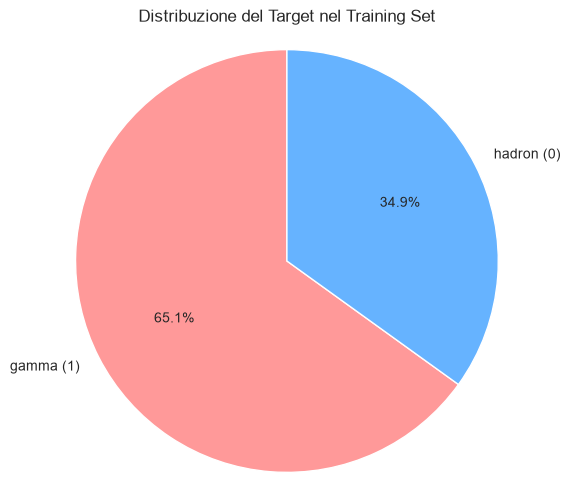
\includegraphics[width=0.55\textwidth]{eda_pie}
	\caption{Distribuzione delle due classi nel training set: i gamma (segnale) sono quasi il doppio degli adroni (fondo).}
	\label{fig:pie}
\end{figure}

Le distribuzioni delle variabili continue (Figura~\ref{fig:hist}) sono prevalentemente asimmetriche verso destra, con densità concentrate sui valori bassi e code lunghe verso destra. Questa asimmetria rende la mediana uno stimatore di tendenza centrale più robusto rispetto alla media. Si nota anche una notevole eterogeneità nelle scale numeriche, che vanno da unità singole a centinaia, il che rende necessaria una successiva normalizzazione.

\begin{figure}[H]\centering
	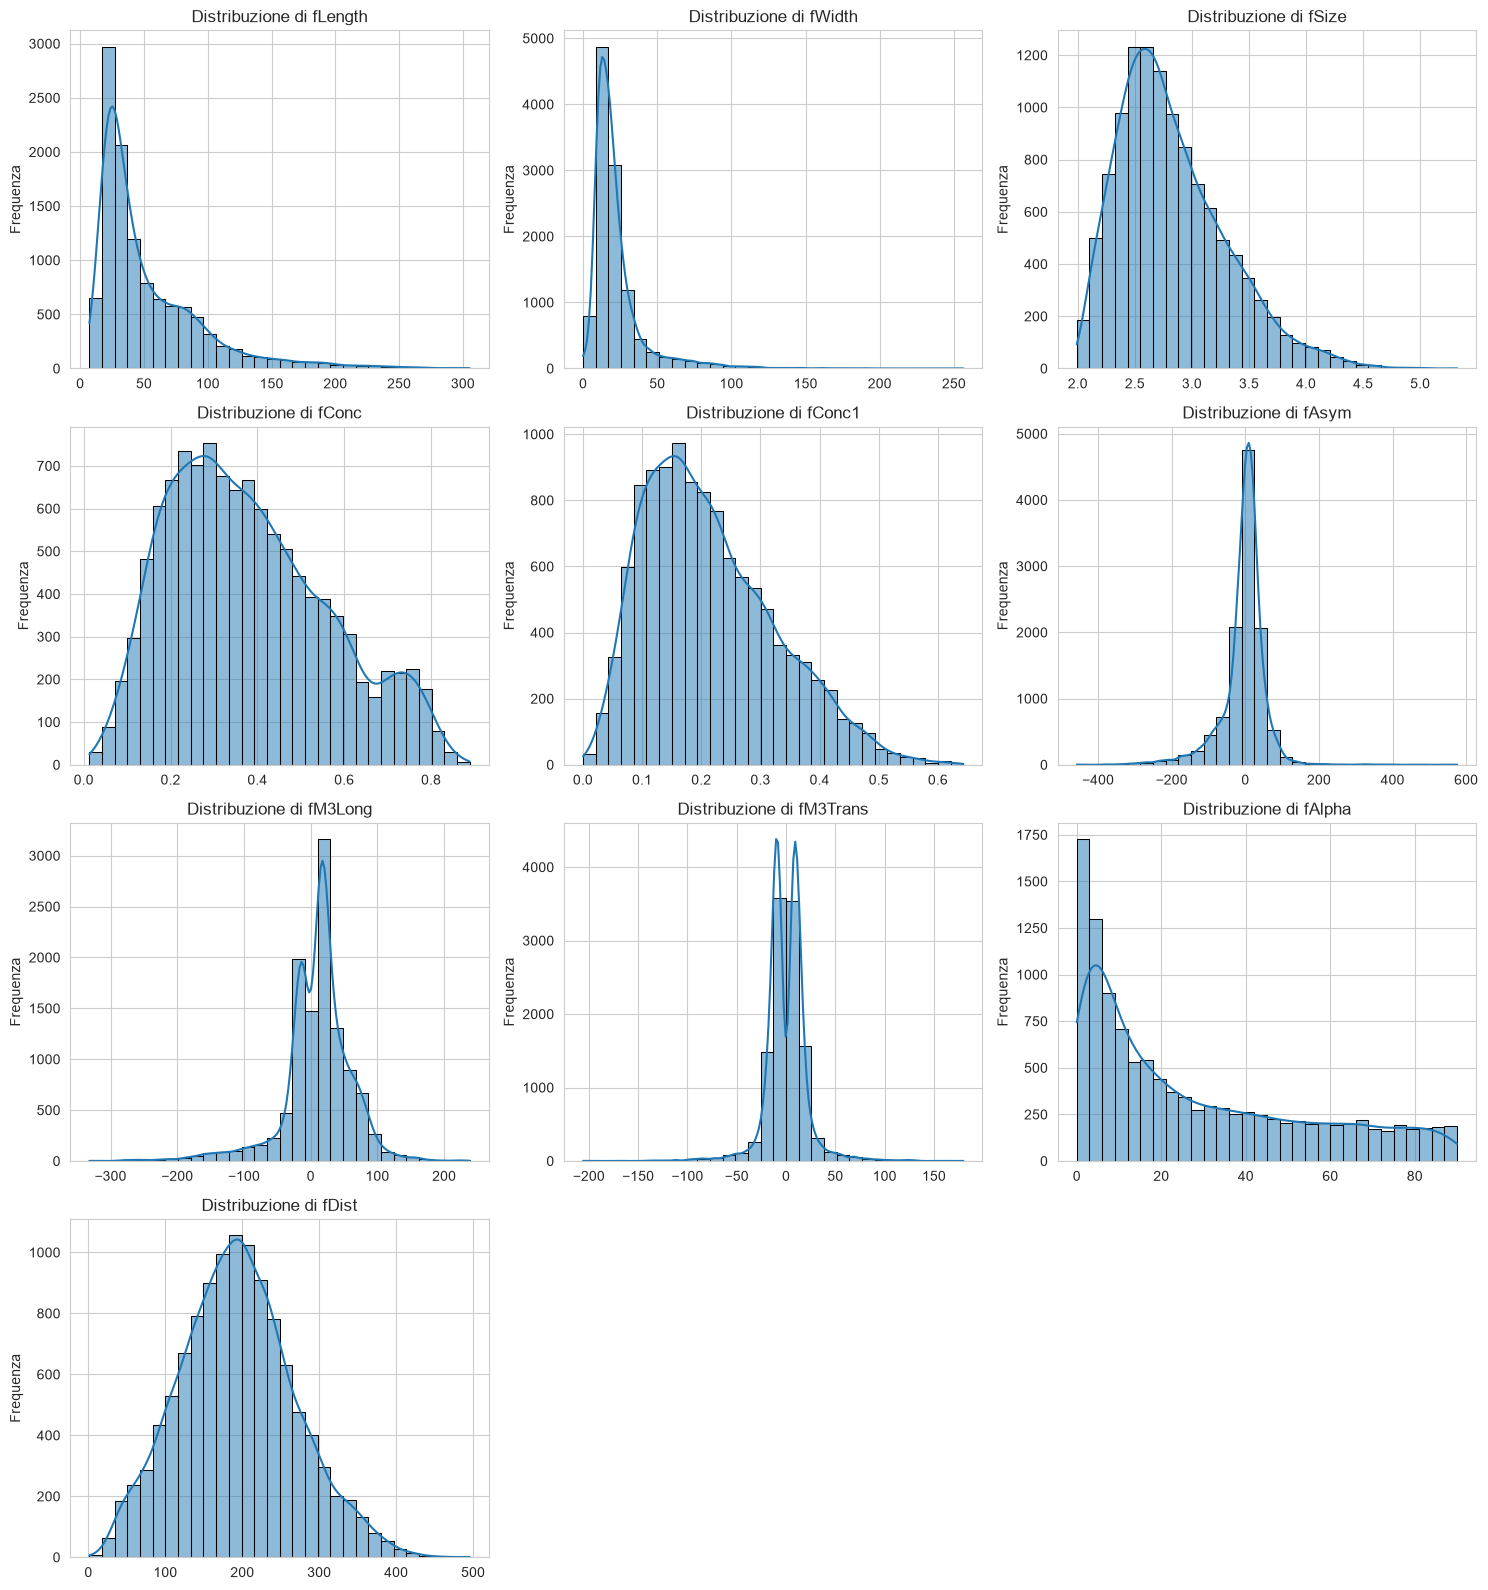
\includegraphics[width=0.95\textwidth]{eda_hist}
	\caption{Istogrammi delle dieci feature continue (training set): distribuzioni asimmetriche, con code lunghe e scale eterogenee.}
	\label{fig:hist}
\end{figure}

I boxplot divisi per classe (Figura~\ref{fig:box}) permettono di valutare il potere discriminante di ciascuna feature. La variabile \texttt{fAlpha} mostra la separazione più netta: i valori dei gamma si concentrano in un intervallo ristretto e basso, mentre quelli degli adroni presentano un'elevata dispersione. Seguono \texttt{fLength}, \texttt{fWidth} e \texttt{fSize}, che offrono un buon contributo informativo. Al contrario, \texttt{fM3Trans} e \texttt{fAsym} mostrano distribuzioni ampiamente sovrapposte tra le due classi. L'informazione utile alla classificazione è quindi concentrata in un sottoinsieme limitato di variabili.

\begin{figure}[H]\centering
	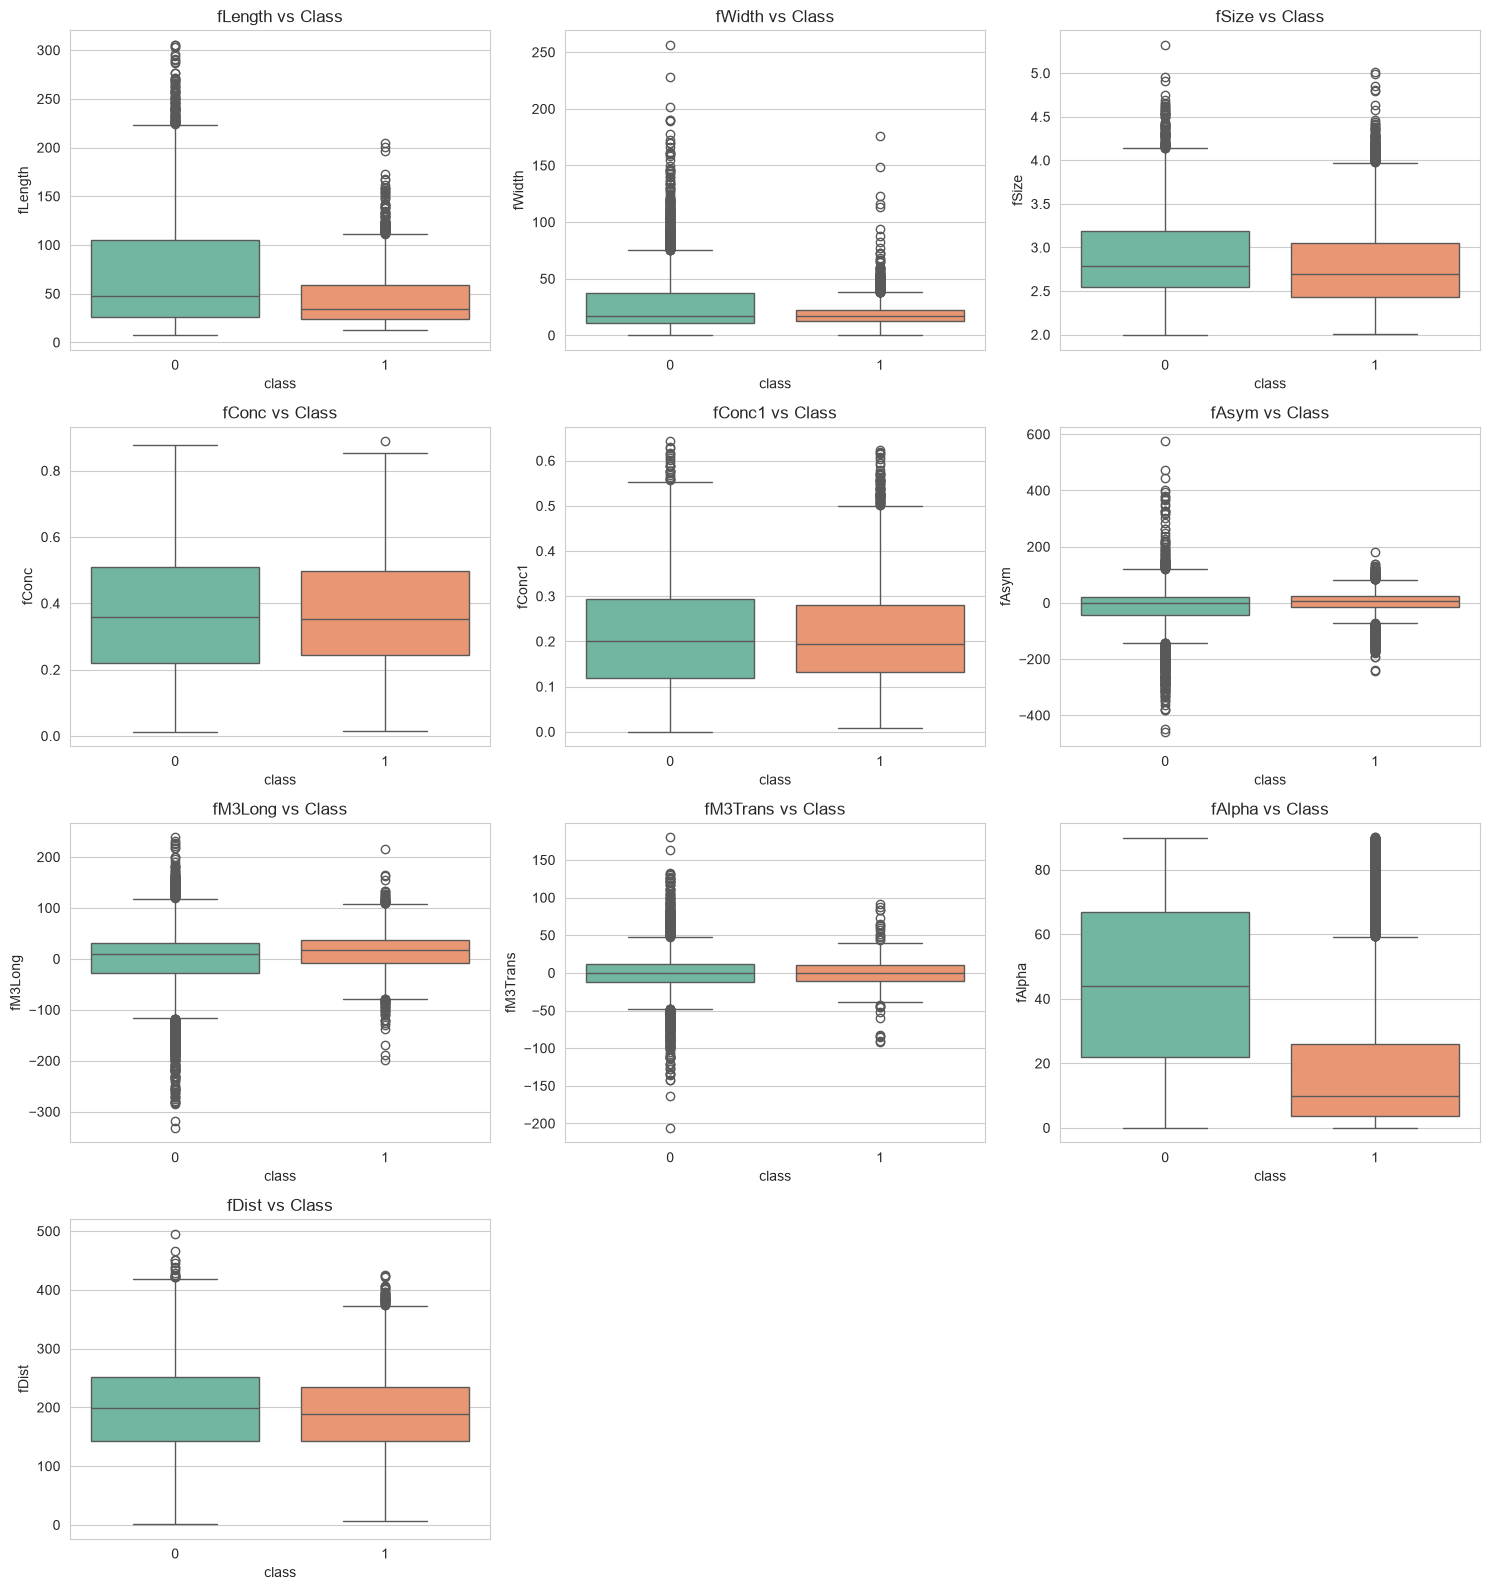
\includegraphics[width=0.95\textwidth]{eda_box}
	\caption{Boxplot di ogni feature per classe (training set): \texttt{fAlpha} è la più discriminante, i momenti trasversali separano poco le classi.}
	\label{fig:box}
\end{figure}

La matrice di correlazione di Pearson (Figura~\ref{fig:corr}) mostra forti dipendenze lineari tra alcune feature. Le variabili \texttt{fConc} e \texttt{fConc1} sono quasi colineari (correlazione di $0{,}98$) e presentano una marcata anticorrelazione con \texttt{fSize} ($-0{,}85$ e $-0{,}81$). Anche il gruppo formato da \texttt{fLength}, \texttt{fWidth} e \texttt{fSize} mostra correlazioni significative, tra $0{,}70$ e $0{,}77$. Questa ridondanza informativa implica che il degrado o l'assenza di una di queste feature possa essere parzialmente compensato dall'informazione contenuta nelle altre. Al contrario, \texttt{fAlpha} è quasi del tutto scorrelata dal resto del dataset: la sua informazione è unica e non recuperabile in caso di corruzione.

\begin{figure}[H]\centering
	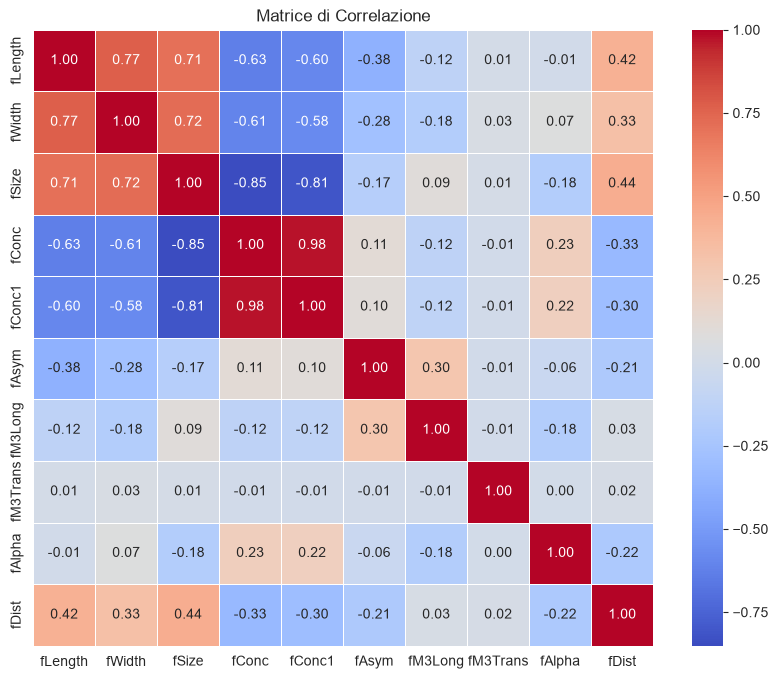
\includegraphics[width=0.82\textwidth]{eda_corr}
	\caption{Matrice di correlazione tra le feature (training set). Spiccano la quasi-ridondanza \texttt{fConc}/\texttt{fConc1} e l'anticorrelazione di \texttt{fSize} con le concentrazioni; \texttt{fAlpha} è quasi scorrelata da tutte.}
	\label{fig:corr}
\end{figure}

% ============================================================
% 5. PREPROCESSING
% ============================================================
\section{Preprocessing: standardizzazione}\label{sec:prep}

L'eterogeneità delle scale numeriche osservata durante l'analisi esplorativa rende indispensabile la standardizzazione delle feature, cioè la traslazione a media nulla e varianza unitaria. Questo passaggio è particolarmente importante per la stabilità e la convergenza delle reti neurali. Senza standardizzazione, le feature con valori molto grandi dominerebbero l'aggiornamento dei gradienti per ragioni di scala e non per il loro effettivo potere predittivo.

Per evitare il data leakage, i parametri di scalatura (media e deviazione standard) sono stati calcolati esclusivamente sul training set. Questi parametri sono stati poi applicati invariati per trasformare il validation e il test set.

% ============================================================
% 6. MODELLI
% ============================================================
\section{Modelli}\label{sec:modelli}

Lo studio confronta tre modelli supervisionati, scelti per rappresentare architetture con livelli crescenti di tolleranza intrinseca al rumore. La Tabella~\ref{tab:modelli} ne riassume i parametri strutturali e gli iperparametri.

La rete neurale Base è un Multi-Layer Perceptron volutamente semplice. Prende in ingresso le dieci feature standardizzate, le elabora attraverso due strati nascosti (da $32$ e $16$ neuroni, entrambi con attivazione ReLU) e produce in uscita un singolo neurone con attivazione sigmoide per stimare la probabilità di classe. L'addestramento usa l'ottimizzatore Adam con tasso di apprendimento $10^{-3}$ e la funzione di costo binary cross-entropy, per $75$ epoche con batch size di $32$. Non avendo alcun meccanismo di regolarizzazione, questa rete rappresenta la baseline ingenua, libera di adattarsi anche ai pattern spuri introdotti dal rumore.

La rete neurale Pro mantiene la stessa architettura della rete Base ma aggiunge quattro meccanismi per contrastare l'overfitting. La regolarizzazione L2 (coefficiente $10^{-4}$ sui pesi degli strati nascosti) penalizza la magnitudo dei pesi, scoraggiando confini decisionali troppo complessi. Il dropout (probabilità $0{,}2$) disabilita casualmente una frazione di neuroni a ogni iterazione, obbligando la rete a distribuire l'apprendimento su più unità. Il class weight bilanciato aumenta la penalizzazione per gli errori sulla classe minoritaria (adroni). Infine, l'early stopping monitora la funzione di costo sul validation set e interrompe l'addestramento se non ci sono miglioramenti per $15$ epoche consecutive, entro un massimo di $150$ epoche, ripristinando i pesi migliori.

Il Random Forest è un ensemble di $200$ alberi decisionali. La sua robustezza viene dal bagging: ogni albero viene addestrato su sottoinsiemi casuali di dati e feature, e le previsioni finali si ottengono per voto maggioritario. Questo meccanismo tende a cancellare la varianza degli errori individuali. Non operando tramite ottimizzazione iterativa, non produce curve di apprendimento; le performance si valutano solo sulle metriche e sulla matrice di confusione finali.

\begin{table}[H]\centering\small
	\caption{Parametri principali dei tre modelli confrontati.}\label{tab:modelli}
	\begin{tabular}{@{}l p{4.6cm} p{6.8cm}@{}}
		\toprule
		\textbf{Modello} & \textbf{Architettura}                    & \textbf{Regolarizzazione / iperparametri}                                                        \\
		\midrule
		NN Base          & Dense(32) $\to$ Dense(16) $\to$ sigmoide & nessuna; Adam $10^{-3}$, 75 epoche, batch 32                                                     \\[4pt]
		NN Pro           & Dense(32) $\to$ Dense(16) $\to$ sigmoide & L2 $10^{-4}$, dropout 0,2, class weight bilanciato, early stopping (patience 15), max 150 epoche \\[4pt]
		Random Forest    & 200 alberi decisionali                   & aggregazione per voto, \texttt{random\_state}=42                                                 \\
		\bottomrule
	\end{tabular}
\end{table}

Per la valutazione complessiva vengono usate quattro metriche calcolate sul test set pulito con soglia decisionale di $0{,}5$. L'accuratezza globale dà un'indicazione generale ma risente dello sbilanciamento delle classi. Per compensare vengono usate l'F1 macro e la Recall macro, che mediano le prestazioni su entrambe le classi penalizzando i modelli che tendono a ignorare gli adroni. L'AUC valuta invece la qualità del ranking probabilistico indipendentemente dalla soglia scelta.

% ============================================================
% 7. BASELINE
% ============================================================
\section{Baseline su dati puliti}\label{sec:baseline}

L'addestramento preliminare sui dati originali stabilisce il riferimento di prestazioni a livello $0\%$ di corruzione. Le metriche ottenute servono da punto di paragone per misurare i futuri degradi. La Tabella~\ref{tab:baseline} riassume i risultati sul test set.

\begin{table}[H]\centering\small
	\caption{Metriche di test dei tre modelli sui dati puliti (riferimento a 0\% di rumore).}\label{tab:baseline}
	\begin{tabular}{lccc}
		\toprule
		\textbf{Modello} & \textbf{Accuratezza} & \textbf{F1 macro} & \textbf{AUC} \\
		\midrule
		NN Base          & 0,8678               & 0,8517            & 0,9214       \\
		NN Pro           & 0,8601               & 0,8468            & 0,9238       \\
		Random Forest    & 0,8785               & 0,8629            & 0,9300       \\
		\bottomrule
	\end{tabular}
\end{table}

I tre modelli partono da prestazioni comparabili, con accuratezza tra l'$86\%$ e l'$88\%$ e AUC tra $0{,}92$ e $0{,}93$. Il Random Forest è il più performante su tutte le metriche. L'accuratezza della rete Pro è leggermente inferiore a quella della rete Base, ma non per colpa di L2 o dropout: il class weight bilanciato, applicato con soglia fissa a $0{,}5$, sposta l'obiettivo verso la classe minoritaria, aumentando la recall sugli adroni (da $0{,}77$ a $0{,}80$) a scapito di una parte della recall sui gamma. L'accuratezza globale scende ma la qualità del ranking probabilistico migliora: la rete Pro ottiene un'AUC leggermente superiore alla Base, a conferma di una maggiore solidità nella stima delle probabilità.

Le matrici di confusione (Figura~\ref{fig:base_cm}) mostrano che tutti i classificatori riconoscono bene i gamma, ma concentrano la maggior parte degli errori sull'identificazione degli adroni. Le curve di apprendimento delle due reti (Figura~\ref{fig:base_curve}) indicano una convergenza regolare. Il divario limitato tra training e validation conferma che non c'è overfitting significativo sui dati non alterati per entrambe le architetture.

\begin{figure}[H]\centering
	\begin{minipage}{0.32\textwidth}\centering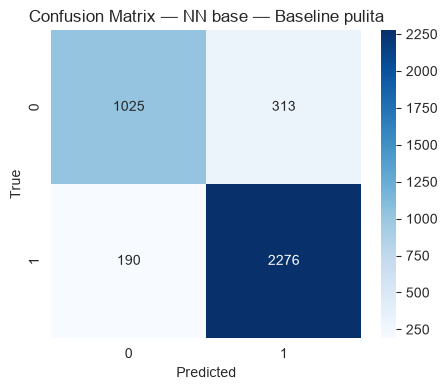
\includegraphics[width=\textwidth]{baseline_nnbase_cm}\end{minipage}\hfill
	\begin{minipage}{0.32\textwidth}\centering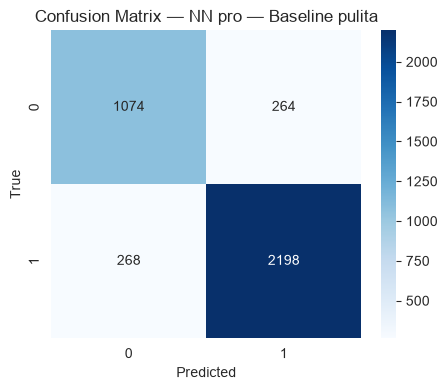
\includegraphics[width=\textwidth]{baseline_nnpro_cm}\end{minipage}\hfill
	\begin{minipage}{0.32\textwidth}\centering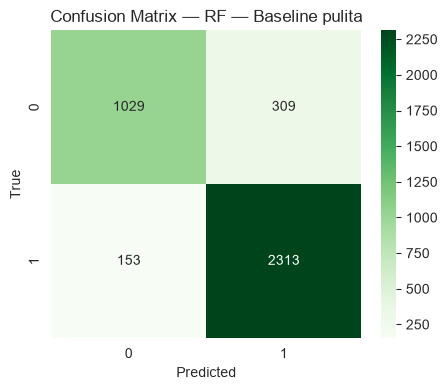
\includegraphics[width=\textwidth]{baseline_rf_cm}\end{minipage}
	\caption{Matrici di confusione sui dati puliti: rete Base, rete Pro e Random Forest (da sinistra a destra). Tutti riconoscono bene i gamma, gli errori si concentrano sugli adroni.}
	\label{fig:base_cm}
\end{figure}

\begin{figure}[H]\centering
	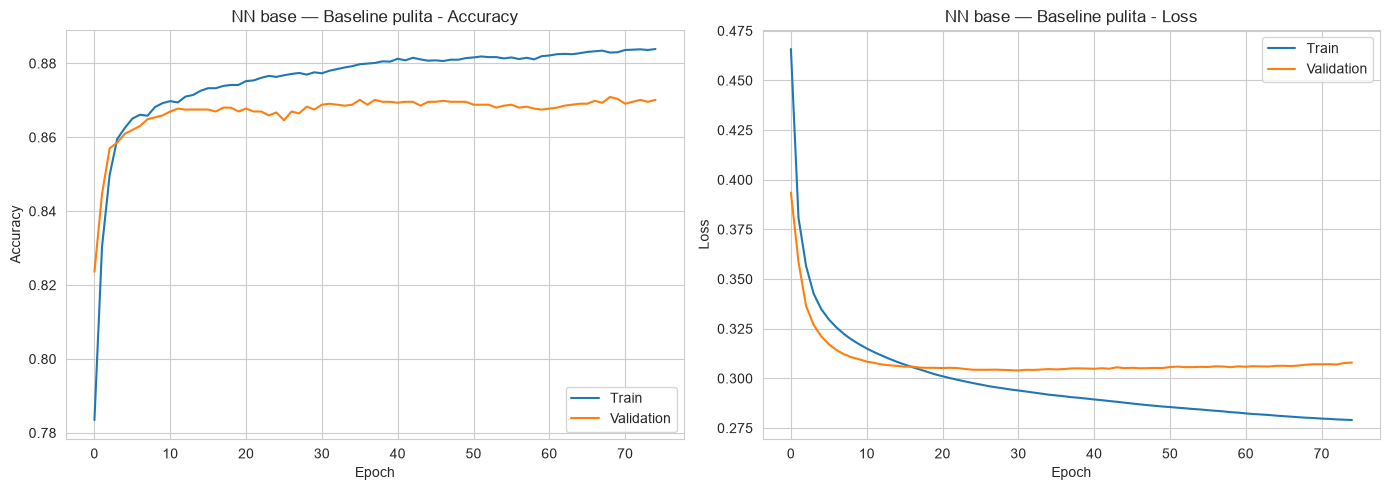
\includegraphics[width=0.9\textwidth]{baseline_nnbase_curve}\\[8pt]
	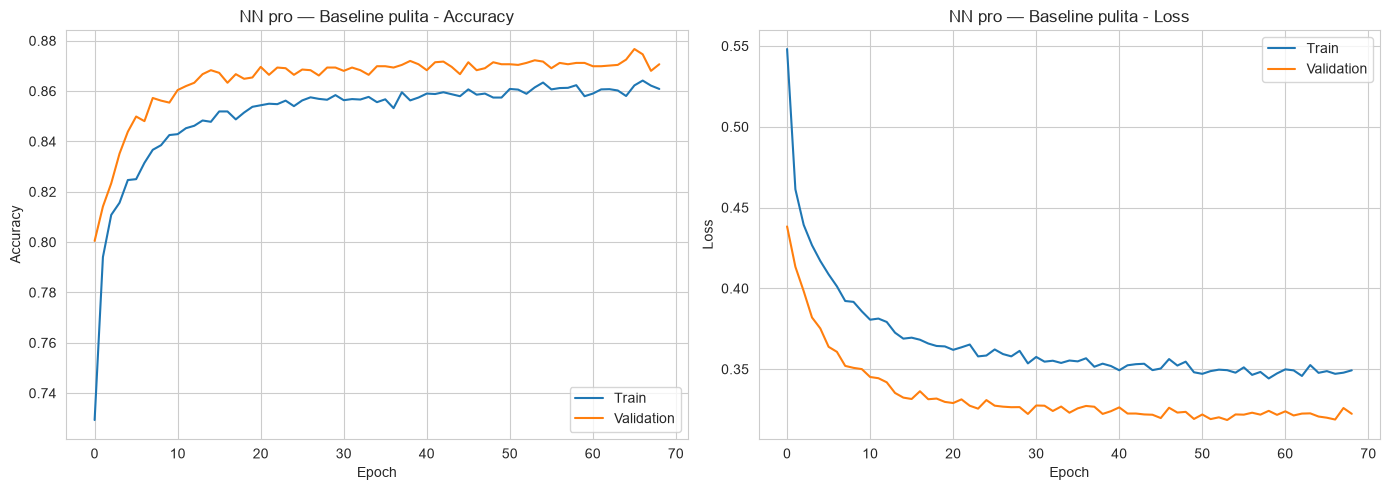
\includegraphics[width=0.9\textwidth]{baseline_nnpro_curve}
	\caption{Curve di accuratezza e loss (train vs validation) sui dati puliti: rete Base (in alto) e rete Pro (in basso).}
	\label{fig:base_curve}
\end{figure}

La feature importance estratta dal Random Forest (Figura~\ref{fig:featimp}) conferma quanto emerso nell'analisi esplorativa. La feature \texttt{fAlpha} domina con un valore di importanza vicino a $0{,}24$, circa una volta e mezza il secondo parametro più rilevante (\texttt{fLength}, $\approx 0{,}15$). Seguono in ordine decrescente \texttt{fLength}, \texttt{fWidth} e \texttt{fSize}.

\begin{figure}[H]\centering
	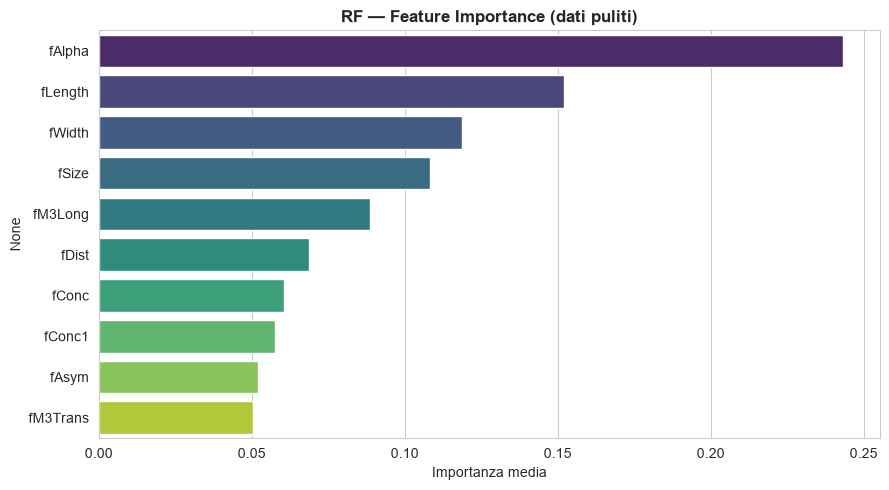
\includegraphics[width=0.86\textwidth]{baseline_featimp}
	\caption{Importanza delle feature secondo il Random Forest sui dati puliti. \texttt{fAlpha} domina, coerentemente con la separabilità osservata nei boxplot.}
	\label{fig:featimp}
\end{figure}

% ============================================================
% 8. METODOLOGIA DEL RUMORE
% ============================================================
\section{Metodologia di iniezione del rumore}\label{sec:rumore}

Il rumore altera esclusivamente il training set, mantenendo intatti validation e test set. In questo modo si valuta correttamente la capacità di generalizzazione di un modello addestrato su dati imperfetti. Per ogni tipo di rumore, i modelli vengono riaddestrati iterativamente a tre livelli di intensità ($10\%$, $25\%$, $40\%$) e le performance vengono sempre misurate sullo stesso test set. L'iniezione del rumore avviene sul training set già standardizzato: trattandosi di perturbazioni additive o monotone, l'operazione è matematicamente equivalente a corrompere i dati originali e standardizzarli in un secondo momento.

Si definiscono sette meccanismi di corruzione.

\subsection{I sette tipi di rumore}

\paragraph{Feature noise (rumore gaussiano).} A ogni singola feature del training set viene sommato un rumore gaussiano a media nulla, con deviazione standard proporzionale al livello percentuale scelto. Poiché le variabili sono già state standardizzate, un rumore al livello $40\%$ introduce fluttuazioni pari al $40\%$ della deviazione standard nativa di ciascuna feature.

\paragraph{Feature noise localizzato.} Qui l'intensità del rumore è fissa a $\sigma = 0{,}35$, mentre varia il numero di feature perturbate. La selezione segue la gerarchia di importanza. Al livello $10\%$ viene perturbata solo \texttt{fAlpha}; al $25\%$ le prime tre variabili discriminanti; al $40\%$ le prime cinque.

\paragraph{Label noise random.} Una percentuale di osservazioni del training set pari al livello scelto subisce l'inversione della variabile target (da $0$ a $1$ e viceversa). Il campionamento è puramente casuale, simulando errori di annotazione distribuiti uniformemente.

\paragraph{Label noise borderline.} L'inversione delle etichette si concentra sulle istanze più ambigue. Dopo aver calcolato i centroidi delle due classi nello spazio standardizzato, si misura la distanza di ogni campione dal centroide della classe opposta. L'inversione colpisce solo i campioni con distanza minima, cioè quelli vicini al confine decisionale.

\paragraph{Missing values.} Singole misurazioni vengono eliminate e sostituite con un valore nullo (\texttt{NaN}), trattando ogni cella come evento indipendente con probabilità pari al livello di corruzione. Non potendo i modelli elaborare dati incompleti, si ricorre all'imputazione. In questa analisi vengono confrontate l'imputazione per media e per mediana della rispettiva feature.

\paragraph{Outlier.} Un numero di campioni proporzionale al livello scelto subisce una corruzione massiva: tutti i valori delle feature per la riga selezionata vengono sostituiti con valori estremi pari a $\pm 5$ deviazioni standard, con segno attribuito casualmente. Le strategie di mitigazione esaminate sono tre: lasciare le istanze invariate; applicare la winsorizzazione (troncamento dei valori ai percentili $5\%$ e $95\%$) per limitare la magnitudo estrema; imputare i dati marcando come mancanti le istanze con z-score assoluto maggiore di $4$ e sostituendole con la mediana. Come riferimento principale viene usata la winsorizzazione, per il suo buon equilibrio tra robustezza e conservazione dei dati.

\paragraph{Missing feature (sensore guasto).} Intere colonne di feature vengono azzerate su tutti i sottoinsiemi (training, validation e test), simulando il guasto totale di un sensore. Anche qui la rimozione segue la gerarchia di importanza decrescente. Al $10\%$ viene inibita \texttt{fAlpha}, al $25\%$ le prime tre variabili predittive, al $40\%$ le prime cinque. Questa configurazione è volutamente pessimistica, perché sopprime le fonti informative principali.

% ============================================================
% 9. RISULTATI PER TIPO DI RUMORE
% ============================================================
\section{Risultati per tipo di rumore}\label{sec:risultati}

L'impatto dei sette disturbi viene analizzato singolarmente, quantificando il degrado prestazionale al crescere della corruzione. Per ciascun test vengono riportate le metriche misurate ai vari livelli e le comparazioni grafiche su accuratezza globale e F1 macro. L'analisi è completata, dove necessario, dalle curve di apprendimento e dalle matrici di confusione nel caso estremo.

% ---------- 9.1 Feature noise ----------
\subsection{Feature noise}

L'aggiunta di rumore gaussiano sulle feature produce un degrado graduale e progressivo. Come mostra la Tabella~\ref{tab:fn}, anche al livello massimo di corruzione ($40\%$) l'accuratezza di tutti i modelli rimane sopra l'$83\%$, con una flessione limitata a tre o quattro punti percentuali rispetto alla baseline. I grafici prestazionali (Figura~\ref{fig:fn_acc}) mostrano curve con pendenza lieve e uniforme sia in accuratezza sia in F1 macro.

\begin{table}[H]\centering\footnotesize
\setlength{\tabcolsep}{4pt}
\caption{Feature noise: metriche al variare del livello di rumore (test set). R$_m$ = recall macro.}\label{tab:fn}
\begin{tabular}{c *{12}{c}}
\toprule
 & \multicolumn{4}{c}{NN Base} & \multicolumn{4}{c}{NN Pro} & \multicolumn{4}{c}{Random Forest}\\
\cmidrule(lr){2-5}\cmidrule(lr){6-9}\cmidrule(lr){10-13}
Rumore & Acc & R$_m$ & F1$_m$ & AUC & Acc & R$_m$ & F1$_m$ & AUC & Acc & R$_m$ & F1$_m$ & AUC \\
\midrule
Pulito & 0.8678 & 0.84 & 0.85 & 0.9214 & 0.8601 & 0.85 & 0.85 & 0.9238 & 0.8785 & 0.85 & 0.86 & 0.9300 \\
10\% & 0.8657 & 0.84 & 0.85 & 0.9187 & 0.8636 & 0.85 & 0.85 & 0.9204 & 0.8646 & 0.83 & 0.84 & 0.9222 \\
25\% & 0.8520 & 0.81 & 0.83 & 0.9074 & 0.8465 & 0.83 & 0.83 & 0.9071 & 0.8494 & 0.81 & 0.82 & 0.9041 \\
40\% & 0.8328 & 0.78 & 0.80 & 0.8941 & 0.8417 & 0.82 & 0.82 & 0.8940 & 0.8318 & 0.78 & 0.80 & 0.8913 \\
\bottomrule
\end{tabular}
\end{table}


\begin{figure}[H]\centering
	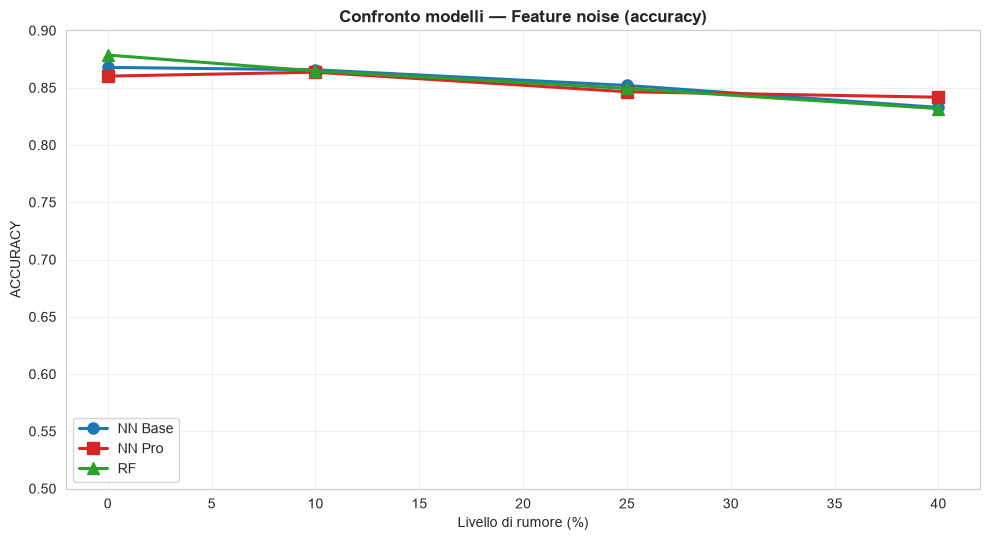
\includegraphics[width=0.86\textwidth]{fn_compare_acc}\\[8pt]
	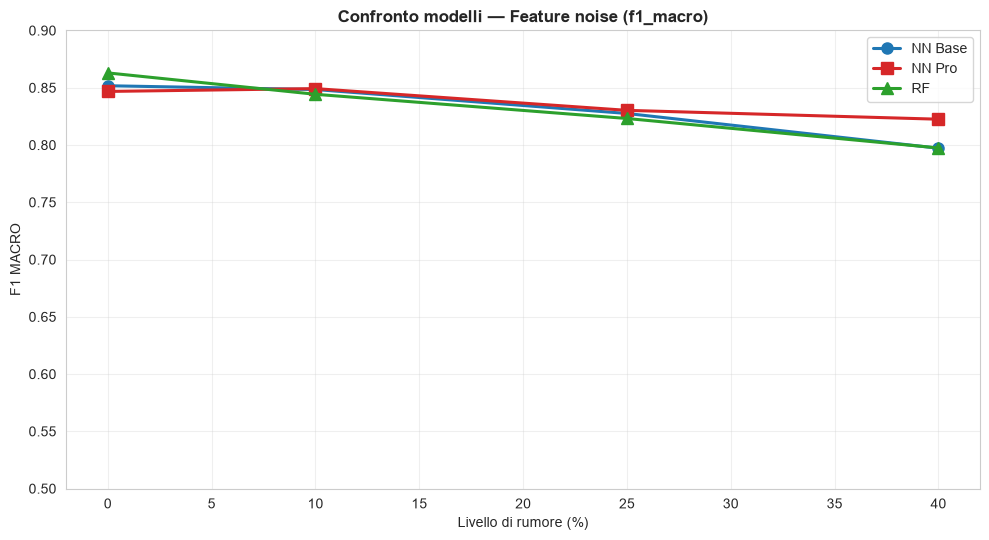
\includegraphics[width=0.86\textwidth]{fn_compare_f1}
	\caption{Feature noise: accuratezza (in alto) e F1 macro (in basso) dei tre modelli al crescere del rumore.}
	\label{fig:fn_acc}
\end{figure}

Al livello $40\%$, la rete Pro raggiunge il valore più alto ($0{,}8417$), distaccando sia la rete Base ($0{,}8328$) sia il Random Forest ($0{,}8318$). Questo risultato conferma l'efficacia della regolarizzazione di fronte a input instabili: la combinazione di L2 e dropout funziona da filtro, impedendo al modello di apprendere le fluttuazioni casuali introdotte. La rete Base, priva di vincoli strutturali, tende invece ad adattarsi al rumore, peggiorando la classificazione su campioni nuovi. Nelle curve di apprendimento dello scenario estremo (Figura~\ref{fig:fn_curve}) si nota come la rete Base mantenga un gap costante tra training e validation loss, mentre la rete Pro tenga le due curve sempre appaiate. In generale, la forte ridondanza tra le feature attenua l'impatto del rumore, perché i modelli possono recuperare parzialmente l'informazione corrotta dalle variabili correlate.

\begin{figure}[H]\centering
	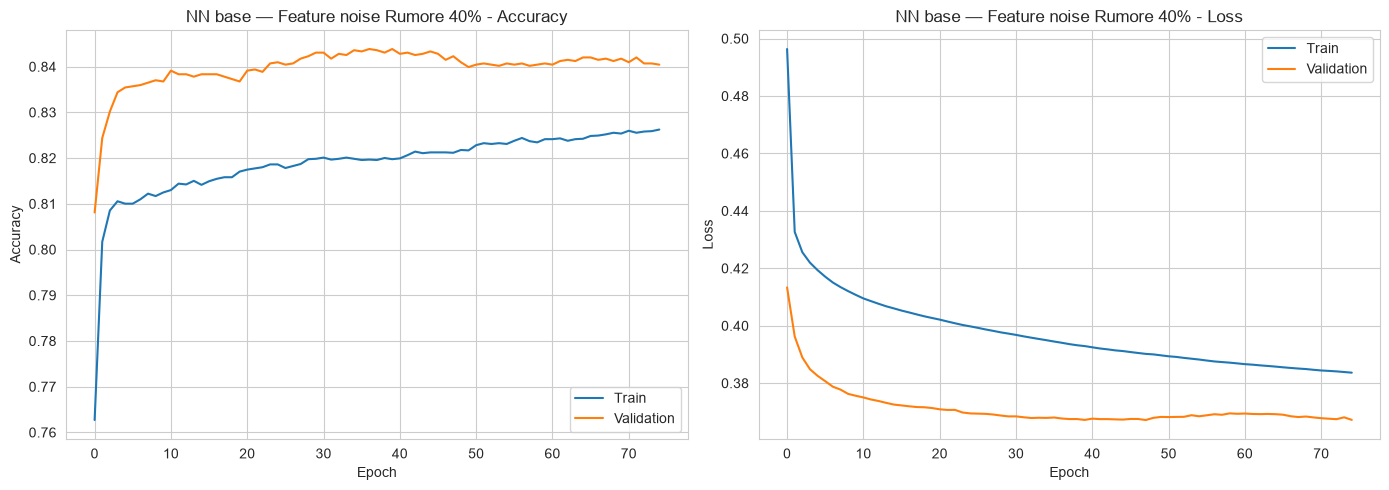
\includegraphics[width=0.9\textwidth]{fn_nnbase_curve40}\\[8pt]
	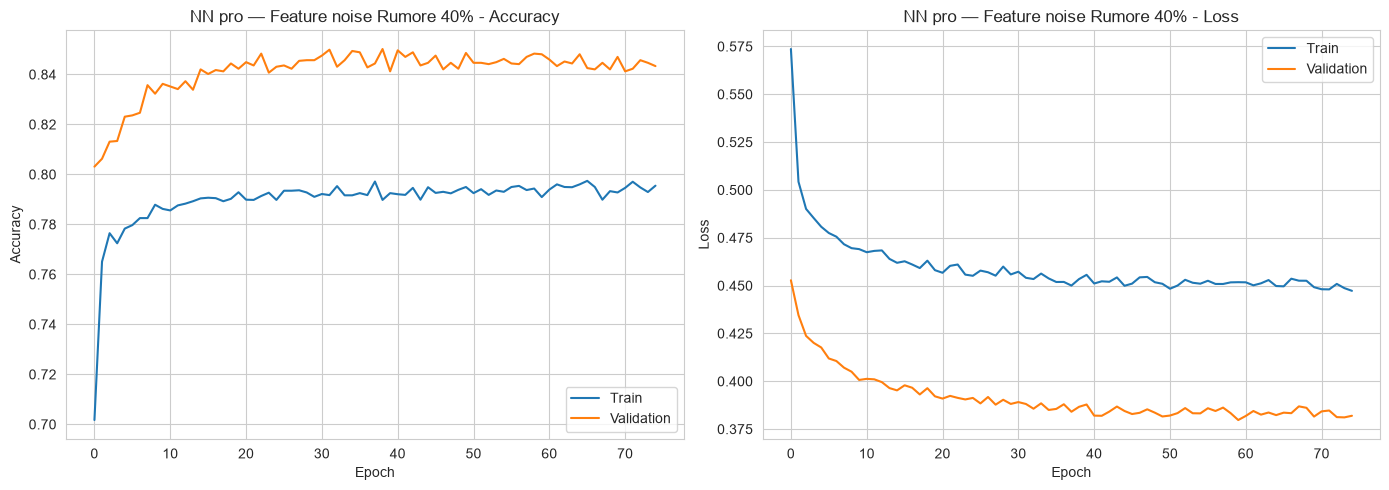
\includegraphics[width=0.9\textwidth]{fn_nnpro_curve40}
	\caption{Feature noise al 40\%: curve di addestramento della rete Base (in alto) e della rete Pro (in basso). Nella rete Pro train e validation restano sovrapposte: la regolarizzazione evita l'adattamento al rumore.}
	\label{fig:fn_curve}
\end{figure}

Il degrado non è però simmetrico tra le classi. Con lo sbilanciamento presente, i modelli tendono a preservare l'accuratezza globale sacrificando il potere predittivo sulla classe rara. Al $40\%$ di rumore, la recall per la classe minoritaria (adroni) della rete Base scende da $0{,}77$ a $0{,}59$, mentre la recall dei gamma sale da $0{,}92$ a $0{,}97$. Questo evidenzia la tendenza a classificare come gamma gli adroni incerti. Il class weight nella rete Pro argina questo fenomeno, mantenendo la recall adronica a $0{,}73$. Le matrici di confusione della rete Base (Figura~\ref{fig:fn_progress}) quantificano chiaramente questo scivolamento.

\begin{figure}[H]\centering
	\begin{minipage}{0.32\textwidth}\centering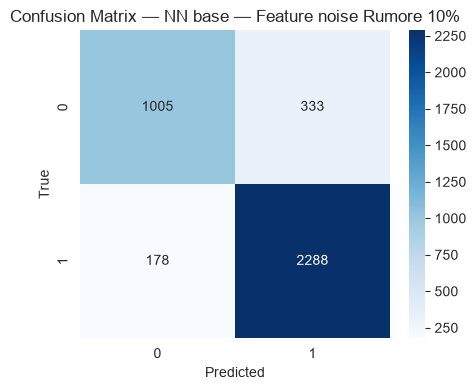
\includegraphics[width=\textwidth]{fn_nnbase_cm10}\end{minipage}\hfill
	\begin{minipage}{0.32\textwidth}\centering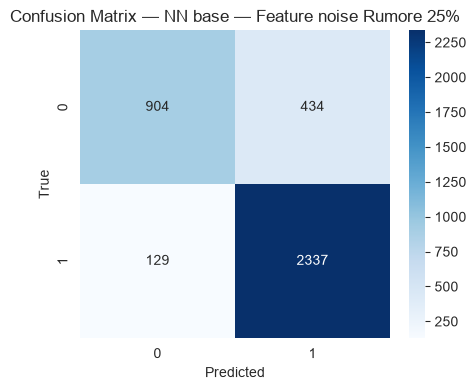
\includegraphics[width=\textwidth]{fn_nnbase_cm25}\end{minipage}\hfill
	\begin{minipage}{0.32\textwidth}\centering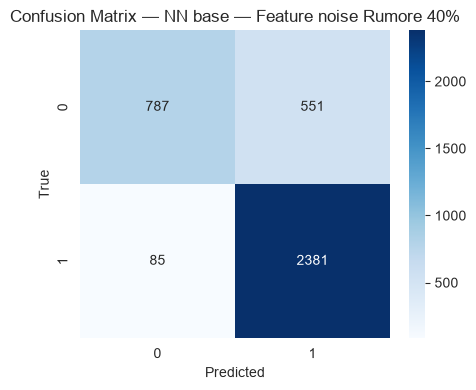
\includegraphics[width=\textwidth]{fn_nnbase_cm40}\end{minipage}
	\caption{Feature noise, rete Base: matrici di confusione al 10\%, 25\% e 40\% (da sinistra a destra). Gli adroni (riga 0) vengono classificati come gamma con frequenza crescente.}
	\label{fig:fn_progress}
\end{figure}

% ---------- 9.1bis Feature noise localizzato ----------
\subsection{Feature noise localizzato}

Concentrare il rumore sulle feature più importanti invece di distribuirlo uniformemente non produce stravolgimenti drammatici (Tabella~\ref{tab:fnloc}). L'intensità della perturbazione è costante a $\sigma = 0{,}35$.

\begin{table}[H]\centering\footnotesize
\setlength{\tabcolsep}{4pt}
\caption{Feature noise localizzato ($\sigma = 0{,}35$) sulle sole feature più importanti: il livello indica quante feature sono colpite (10\%$\to$top-1, 25\%$\to$top-3, 40\%$\to$top-5). R$_m$ = recall macro.}\label{tab:fnloc}
\begin{tabular}{c *{12}{c}}
\toprule
 & \multicolumn{4}{c}{NN Base} & \multicolumn{4}{c}{NN Pro} & \multicolumn{4}{c}{Random Forest}\\
\cmidrule(lr){2-5}\cmidrule(lr){6-9}\cmidrule(lr){10-13}
Rumore & Acc & R$_m$ & F1$_m$ & AUC & Acc & R$_m$ & F1$_m$ & AUC & Acc & R$_m$ & F1$_m$ & AUC \\
\midrule
Pulito & 0.8678 & 0.84 & 0.85 & 0.9214 & 0.8601 & 0.85 & 0.85 & 0.9238 & 0.8785 & 0.85 & 0.86 & 0.9300 \\
10\% & 0.8651 & 0.84 & 0.85 & 0.9211 & 0.8651 & 0.85 & 0.85 & 0.9243 & 0.8743 & 0.85 & 0.86 & 0.9274 \\
25\% & 0.8523 & 0.82 & 0.83 & 0.9043 & 0.8478 & 0.83 & 0.83 & 0.9058 & 0.8533 & 0.82 & 0.83 & 0.9056 \\
40\% & 0.8452 & 0.81 & 0.82 & 0.8991 & 0.8386 & 0.82 & 0.82 & 0.8973 & 0.8389 & 0.79 & 0.81 & 0.8931 \\
\bottomrule
\end{tabular}
\end{table}


\begin{figure}[H]\centering
	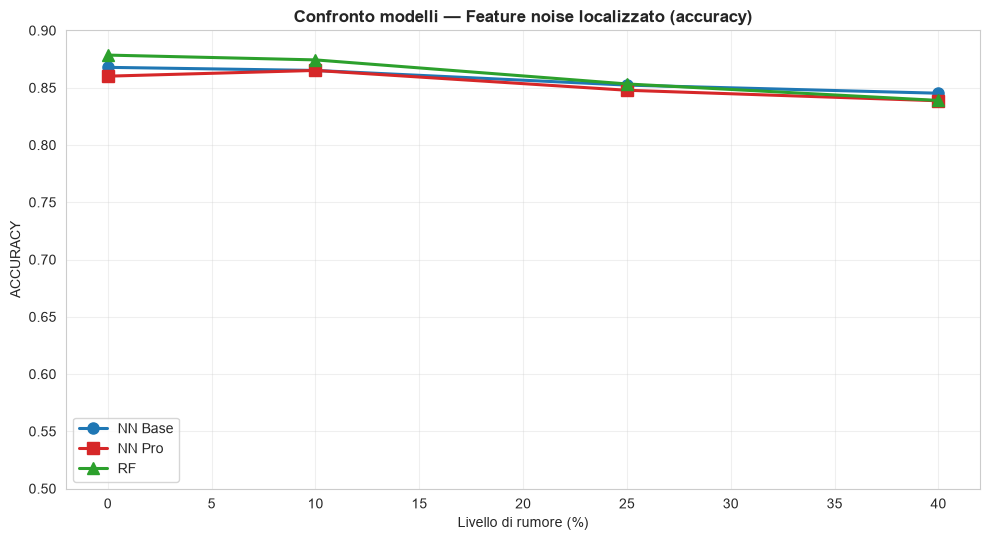
\includegraphics[width=0.86\textwidth]{fnloc_compare_acc}\\[8pt]
	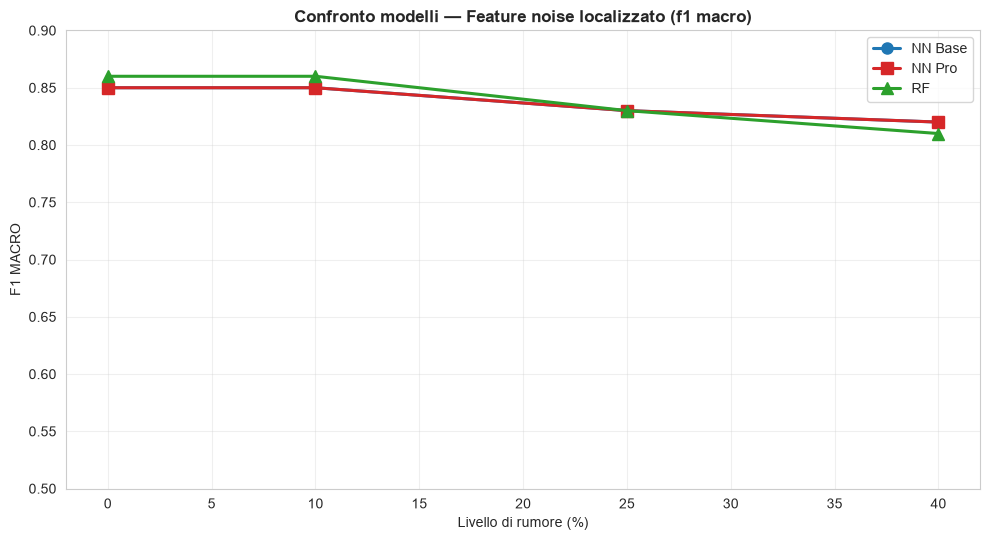
\includegraphics[width=0.86\textwidth]{fnloc_compare_f1}
	\caption{Feature noise localizzato: accuratezza (in alto) e F1 macro (in basso). Le curve restano vicine e quasi piatte.}
	\label{fig:fnloc_acc}
\end{figure}

Il degrado rimane lieve anche perturbando le cinque feature principali. Al livello $40\%$, tutti i classificatori restano sopra l'$83\%$ di accuratezza. L'analisi per classe (Figura~\ref{fig:fnloc_cm}) conferma le dinamiche già osservate: al livello apicale, la recall adronica della rete Base si ferma a $0{,}67$, mentre i pesi bilanciati della rete Pro la tengono a $0{,}75$.

L'andamento delle curve di apprendimento (Figura~\ref{fig:fnloc_curve}) non si discosta da quello visto nel rumore diffuso. Il confronto più significativo emerge mettendo a confronto questo scenario con quello della rimozione completa delle feature: perturbando \texttt{fAlpha} l'accuratezza della rete Base scende a $0{,}8651$, mentre azzerandola del tutto calerà a $0{,}8215$. La perturbazione degrada la qualità dell'informazione senza annullarla, e la rete riesce a recuperarne una parte attraverso le variabili correlate.

\begin{figure}[H]\centering
	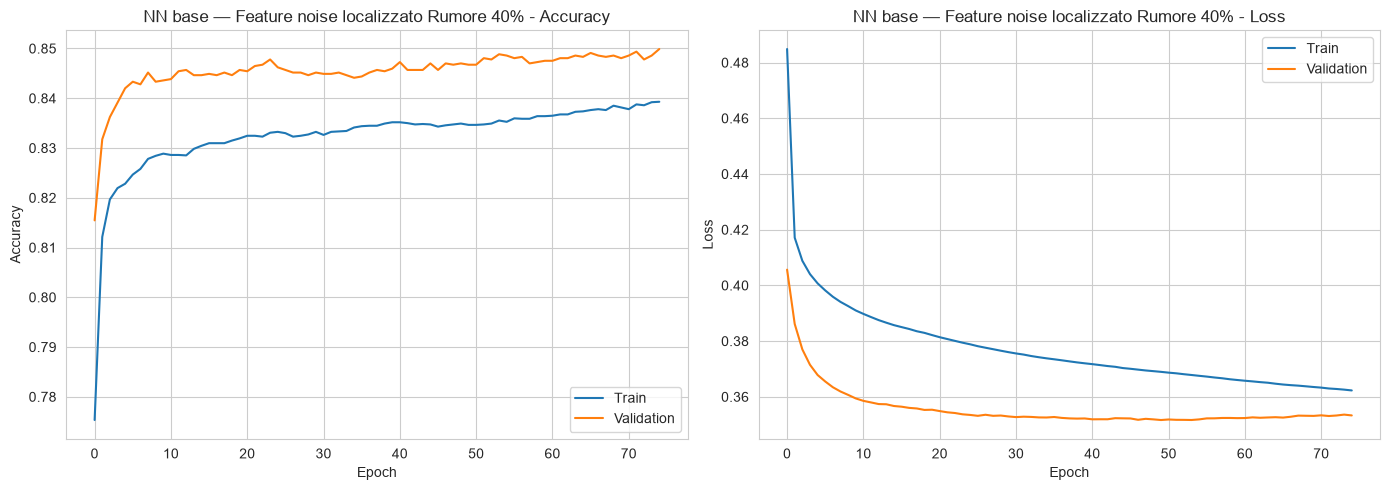
\includegraphics[width=0.9\textwidth]{fnloc_nnbase_curve40}\\[8pt]
	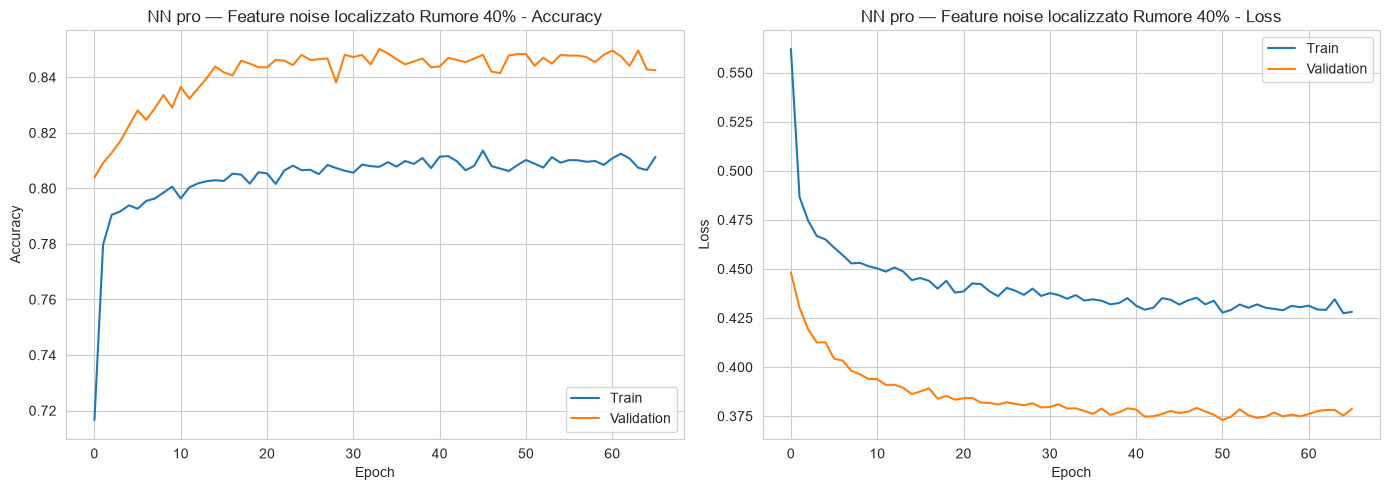
\includegraphics[width=0.9\textwidth]{fnloc_nnpro_curve40}
	\caption{Feature noise localizzato al 40\%: curve di addestramento. L'andamento ricalca il feature noise globale, senza overfitting.}
	\label{fig:fnloc_curve}
\end{figure}

\begin{figure}[H]\centering
	\begin{minipage}{0.49\textwidth}\centering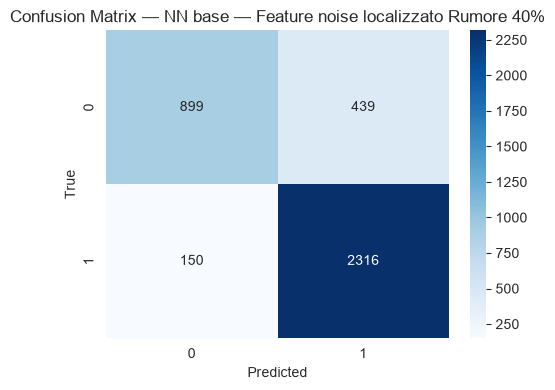
\includegraphics[width=\textwidth]{fnloc_nnbase_cm40}\end{minipage}\hfill
	\begin{minipage}{0.49\textwidth}\centering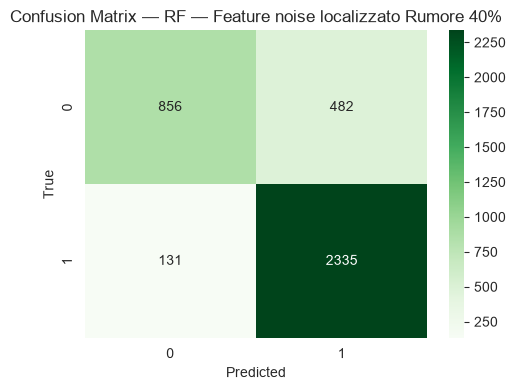
\includegraphics[width=\textwidth]{fnloc_rf_cm40}\end{minipage}
	\caption{Feature noise localizzato al 40\%: matrici di confusione della rete Base (sinistra) e del Random Forest (destra).}
	\label{fig:fnloc_cm}
\end{figure}

% ---------- 9.2 Label noise random ----------
\subsection{Label noise random}

Alterare casualmente la variabile target produce dinamiche molto diverse da quelle viste sulle feature. Fino al $25\%$ i classificatori mantengono metriche adeguate, ma al $40\%$ il calo diventa drammatico. Come mostra la Tabella~\ref{tab:lnr}, l'accuratezza della rete Base crolla a $0{,}7419$ e quella del Random Forest a $0{,}7179$. La rete Pro mostra invece una resilienza notevole, mantenendosi a $0{,}8044$ (Figura~\ref{fig:lnr_acc}).

\begin{table}[H]\centering\footnotesize
\setlength{\tabcolsep}{4pt}
\caption{Label noise random: metriche al variare del livello di rumore (test set). R$_m$ = recall macro.}\label{tab:lnr}
\begin{tabular}{c *{12}{c}}
\toprule
 & \multicolumn{4}{c}{NN Base} & \multicolumn{4}{c}{NN Pro} & \multicolumn{4}{c}{Random Forest}\\
\cmidrule(lr){2-5}\cmidrule(lr){6-9}\cmidrule(lr){10-13}
Rumore & Acc & R$_m$ & F1$_m$ & AUC & Acc & R$_m$ & F1$_m$ & AUC & Acc & R$_m$ & F1$_m$ & AUC \\
\midrule
Pulito & 0.8678 & 0.84 & 0.85 & 0.9214 & 0.8601 & 0.85 & 0.85 & 0.9238 & 0.8785 & 0.85 & 0.86 & 0.9300 \\
10\% & 0.8623 & 0.83 & 0.84 & 0.9128 & 0.8570 & 0.84 & 0.84 & 0.9200 & 0.8767 & 0.85 & 0.86 & 0.9214 \\
25\% & 0.8410 & 0.82 & 0.82 & 0.8882 & 0.8378 & 0.83 & 0.83 & 0.9081 & 0.8399 & 0.81 & 0.82 & 0.8884 \\
40\% & 0.7419 & 0.68 & 0.69 & 0.7513 & 0.8044 & 0.79 & 0.79 & 0.8677 & 0.7179 & 0.70 & 0.70 & 0.7673 \\
\bottomrule
\end{tabular}
\end{table}


\begin{figure}[H]\centering
	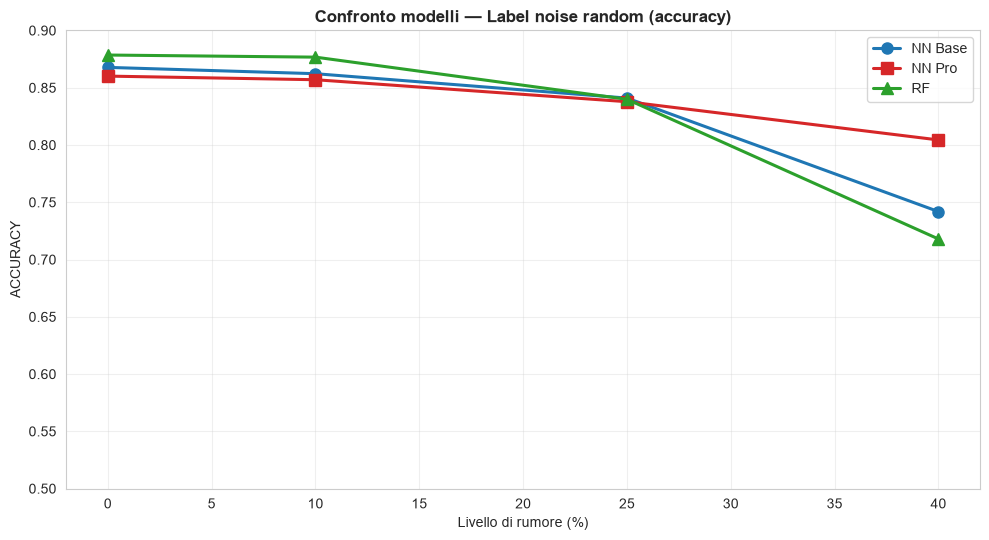
\includegraphics[width=0.86\textwidth]{lnr_compare_acc}\\[8pt]
	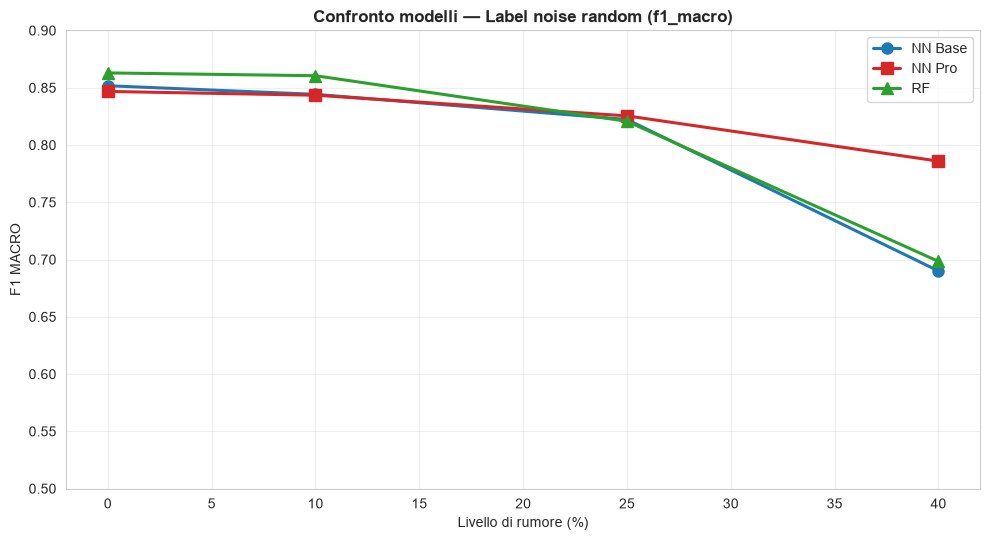
\includegraphics[width=0.86\textwidth]{lnr_compare_f1}
	\caption{Label noise random: accuratezza e F1 macro. Al 40\% la rete Pro si stacca verso l'alto, mentre Base e Random Forest crollano.}
	\label{fig:lnr_acc}
\end{figure}

La causa di questa divergenza è visibile nelle curve di apprendimento (Figura~\ref{fig:lnr_curve}). La rete Base interiorizza le annotazioni errate, portando la curva di training vicino all'$88\%$ mentre la validation loss peggiora costantemente sulle etichette originali e pulite. Al contrario, l'early stopping della rete Pro, che monitora la loss sul validation set non corrotto, interrompe in tempo l'addestramento. Fermando i pesi a uno stadio prematuro ma ottimale, protegge il modello dalla memorizzazione di massa del rumore e mantiene la validation accuracy vicina all'$82\%$.

\begin{figure}[H]\centering
	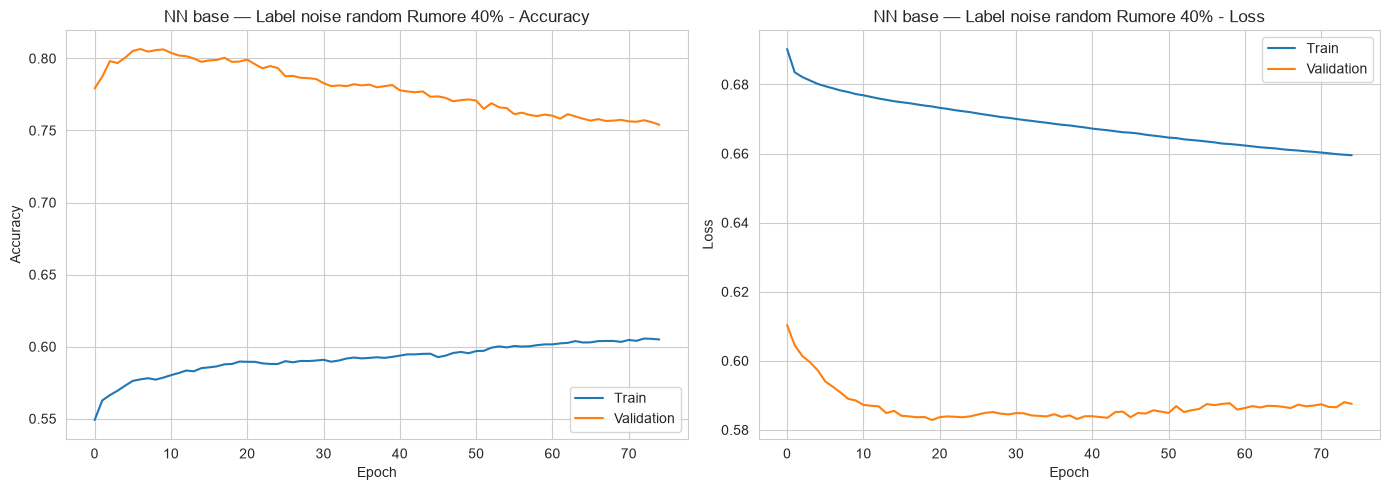
\includegraphics[width=0.9\textwidth]{lnr_nnbase_curve40}\\[8pt]
	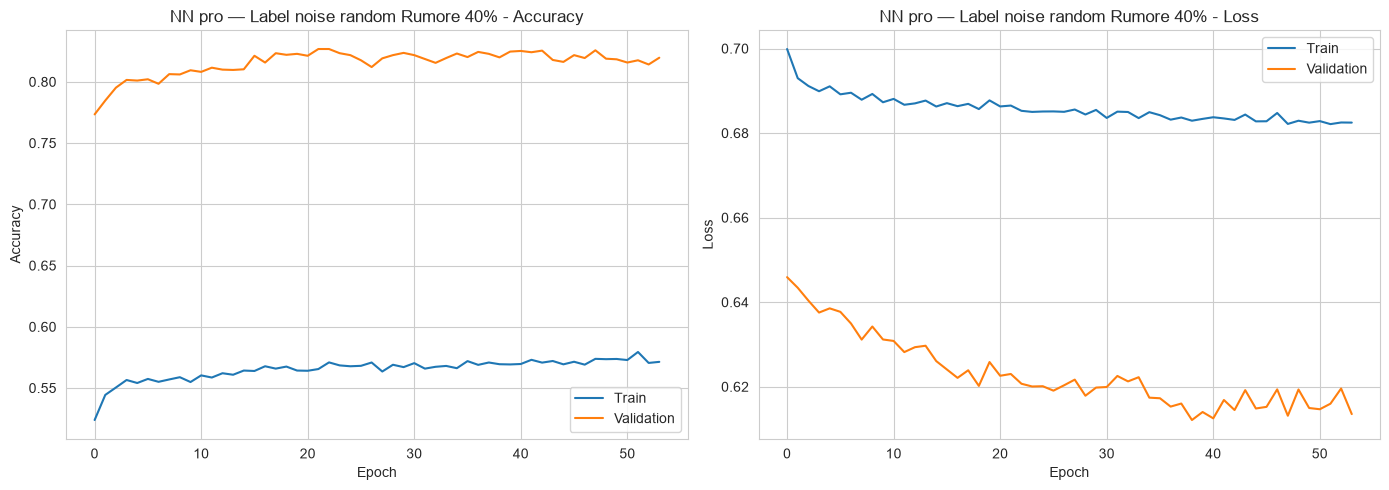
\includegraphics[width=0.9\textwidth]{lnr_nnpro_curve40}
	\caption{Label noise random al 40\%: la Base memorizza le etichette corrotte (train sale, validation scende); la Pro, fermata dall'early stopping, mantiene alta la validation.}
	\label{fig:lnr_curve}
\end{figure}

Non avendo meccanismi iterativi vincolati a set di validazione puliti, il Random Forest assorbe i target errati nei nodi di divisione. La distribuzione uniforme dell'errore (Figura~\ref{fig:lnr_cm}) lo conferma, producendo decrementi simili sulle metriche di entrambe le classi.

\begin{figure}[H]\centering
	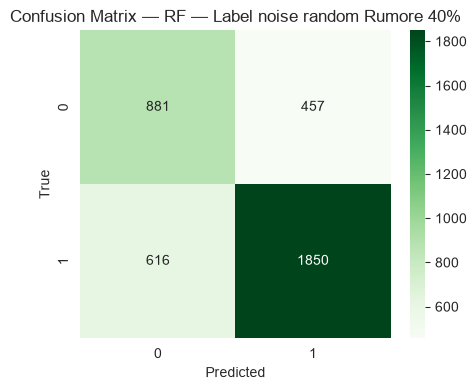
\includegraphics[width=0.52\textwidth]{lnr_rf_cm40}
	\caption{Label noise random al 40\%: matrice di confusione del Random Forest. Gli errori aumentano su entrambe le classi.}
	\label{fig:lnr_cm}
\end{figure}

% ---------- 9.3 Label noise borderline ----------
\subsection{Label noise borderline}

Corrompere selettivamente le istanze vicine ai confini decisionali è il tipo di disturbo più distruttivo tra quelli testati. Le metriche calano in modo marcato già al $25\%$. Al $40\%$, l'accuratezza di tutti i modelli converge intorno al $60\%$, scendendo sotto la soglia di un classificatore che prevede sempre la classe maggioritaria ($\approx 65\%$): il rumore borderline rende i modelli attivamente fuorvianti (Tabella~\ref{tab:lnb} e Figura~\ref{fig:lnb_acc}).

\begin{table}[H]\centering\footnotesize
\setlength{\tabcolsep}{4pt}
\caption{Label noise borderline: metriche al variare del livello di rumore (test set). R$_m$ = recall macro.}\label{tab:lnb}
\begin{tabular}{c *{12}{c}}
\toprule
 & \multicolumn{4}{c}{NN Base} & \multicolumn{4}{c}{NN Pro} & \multicolumn{4}{c}{Random Forest}\\
\cmidrule(lr){2-5}\cmidrule(lr){6-9}\cmidrule(lr){10-13}
Rumore & Acc & R$_m$ & F1$_m$ & AUC & Acc & R$_m$ & F1$_m$ & AUC & Acc & R$_m$ & F1$_m$ & AUC \\
\midrule
Pulito & 0.8678 & 0.84 & 0.85 & 0.9214 & 0.8601 & 0.85 & 0.85 & 0.9238 & 0.8785 & 0.85 & 0.86 & 0.9300 \\
10\% & 0.8252 & 0.79 & 0.80 & 0.8680 & 0.8352 & 0.82 & 0.82 & 0.8915 & 0.8383 & 0.80 & 0.81 & 0.8886 \\
25\% & 0.7326 & 0.71 & 0.71 & 0.7879 & 0.7403 & 0.73 & 0.72 & 0.8265 & 0.7387 & 0.72 & 0.72 & 0.8043 \\
40\% & 0.6002 & 0.61 & 0.59 & 0.6656 & 0.6354 & 0.63 & 0.62 & 0.7084 & 0.6094 & 0.62 & 0.60 & 0.6774 \\
\bottomrule
\end{tabular}
\end{table}


\begin{figure}[H]\centering
	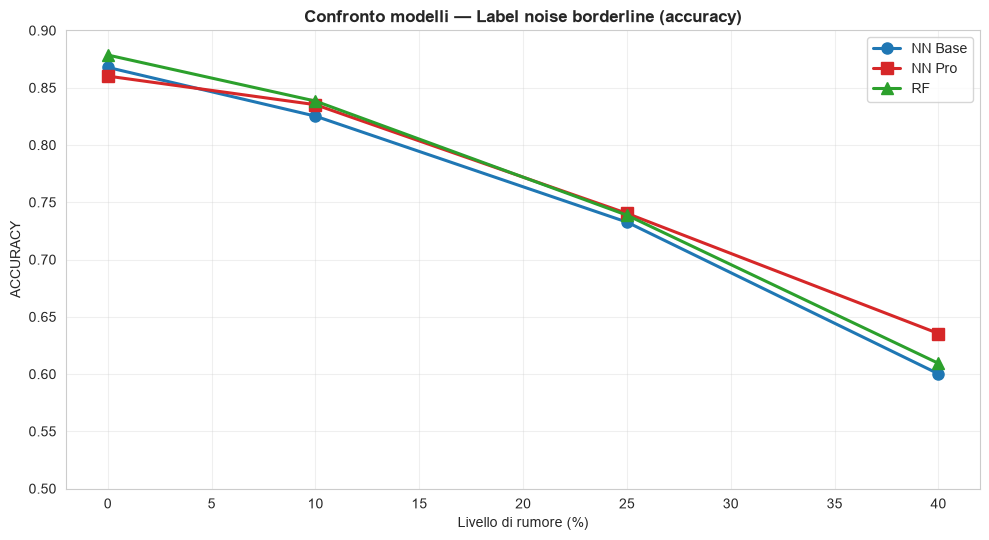
\includegraphics[width=0.86\textwidth]{lnb_compare_acc}\\[8pt]
	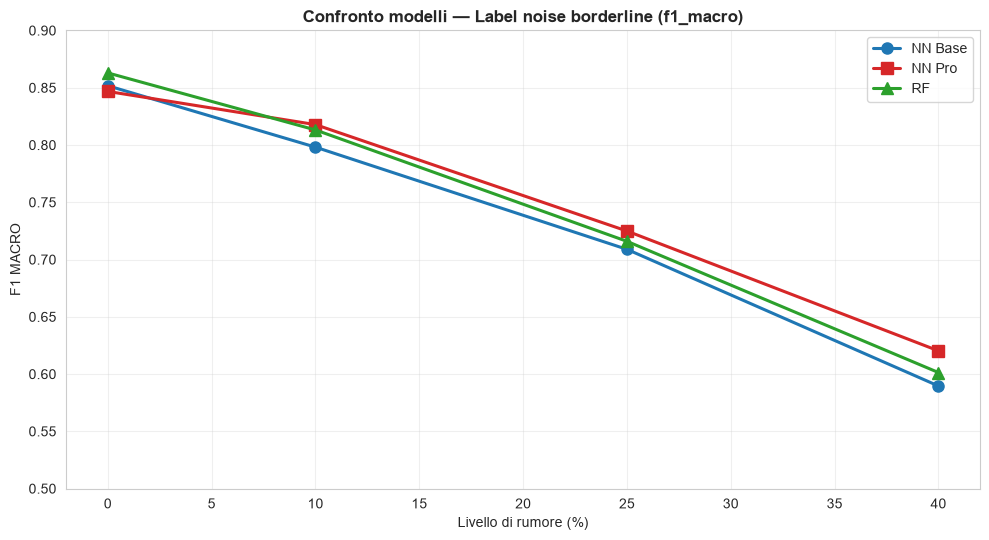
\includegraphics[width=0.86\textwidth]{lnb_compare_f1}
	\caption{Label noise borderline: al 40\% tutti i modelli convergono attorno al 60\%, indicando il collasso predittivo.}
	\label{fig:lnb_acc}
\end{figure}

A parità di percentuale rispetto al label noise random, il disturbo borderline ha una distruttività molto maggiore. Invertire sistematicamente le etichette dei campioni vicini al confine tra le classi sposta il confine decisionale in modo macroscopico. Le curve di apprendimento della rete Pro (Figura~\ref{fig:lnb_curve}) non mostrano alcun vantaggio dalla regolarizzazione né dall'early stopping: quando il confine decisionale è corrotto in modo massiccio, nessun meccanismo di profilassi riesce a recuperare la separazione tra le classi.

\begin{figure}[H]\centering
	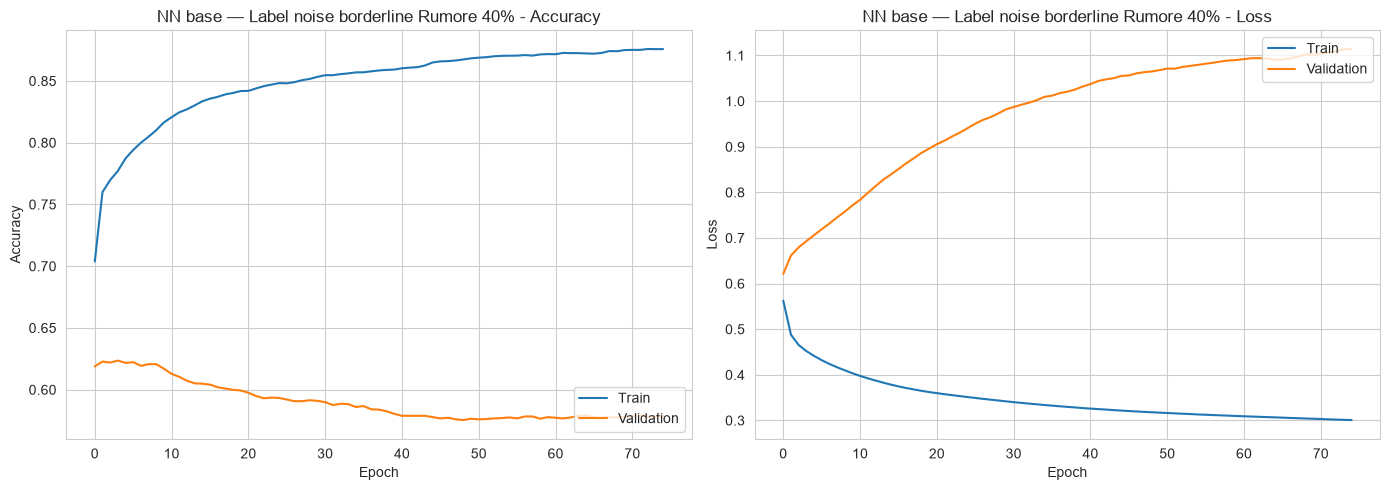
\includegraphics[width=0.9\textwidth]{lnb_nnbase_curve40}\\[8pt]
	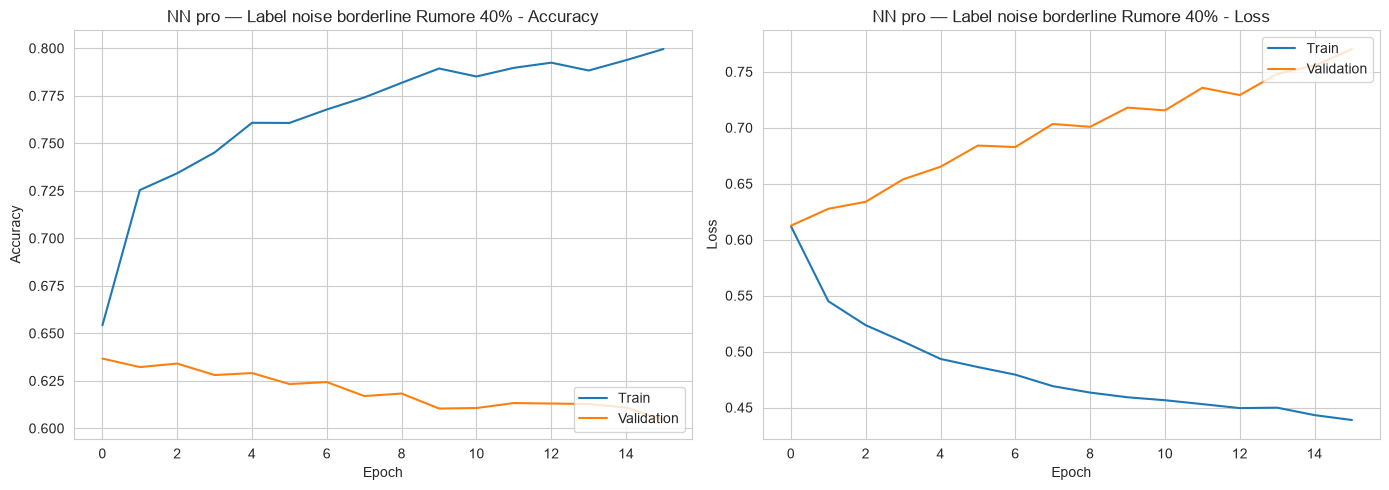
\includegraphics[width=0.9\textwidth]{lnb_nnpro_curve40}
	\caption{Label noise borderline al 40\%: anche la validation della rete Pro crolla, a causa della falsificazione strutturale del confine decisionale.}
	\label{fig:lnb_curve}
\end{figure}

A differenza del rumore sulle feature, in questo scenario il danno si distribuisce in modo sostanzialmente bilanciato tra le due classi. Pur essendo i flip più numerosi sulla classe maggioritaria (gamma), l'effetto sul test porta a un aumento degli errori su entrambe le classi (Figura~\ref{fig:lnb_cm}).

\begin{figure}[H]\centering
	\begin{minipage}{0.49\textwidth}\centering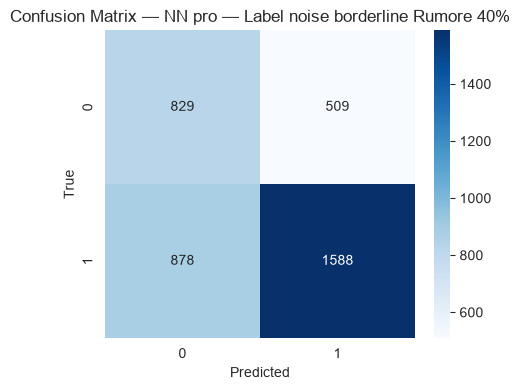
\includegraphics[width=\textwidth]{lnb_nnpro_cm40}\end{minipage}\hfill
	\begin{minipage}{0.49\textwidth}\centering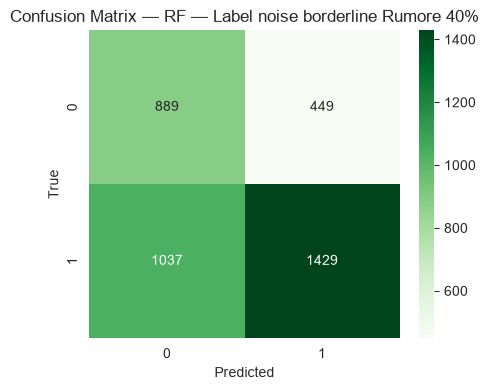
\includegraphics[width=\textwidth]{lnb_rf_cm40}\end{minipage}
	\caption{Label noise borderline al 40\%: matrici di confusione della rete Pro (sinistra) e del Random Forest (destra). Errori diffusi in modo simmetrico.}
	\label{fig:lnb_cm}
\end{figure}

% ---------- 9.4 Missing values ----------
\subsection{Missing values}

La sostituzione di singoli attributi con valori nulli produce peggioramenti lineari e proporzionali, a patto di usare tecniche di ripristino adeguate. Con l'imputazione per mediana (variante canonica), le metriche globali si mantengono tra l'$82\%$ e l'$85\%$ (Tabella~\ref{tab:mv}). In questo scenario il Random Forest mostra il minor calo, con accuratezza massima pari a $0{,}8528$ (Figura~\ref{fig:mv_acc}).

\begin{table}[H]\centering\footnotesize
\caption{Missing values (imputazione con mediana): metriche al variare del tasso di valori mancanti.}\label{tab:mv}
\begin{tabular}{c *{9}{c}}
\toprule
 & \multicolumn{3}{c}{NN Base} & \multicolumn{3}{c}{NN Pro} & \multicolumn{3}{c}{Random Forest}\\
\cmidrule(lr){2-4}\cmidrule(lr){5-7}\cmidrule(lr){8-10}
Rumore & Acc & F1$_m$ & AUC & Acc & F1$_m$ & AUC & Acc & F1$_m$ & AUC \\
\midrule
Pulito & 0.8678 & 0.85 & 0.9214 & 0.8601 & 0.85 & 0.9238 & 0.8785 & 0.86 & 0.9300 \\
10\% & 0.8423 & 0.82 & 0.8947 & 0.8375 & 0.82 & 0.9002 & 0.8559 & 0.84 & 0.9051 \\
25\% & 0.8123 & 0.79 & 0.8645 & 0.7978 & 0.78 & 0.8649 & 0.8270 & 0.80 & 0.8750 \\
40\% & 0.7792 & 0.74 & 0.8266 & 0.7650 & 0.75 & 0.8319 & 0.8068 & 0.78 & 0.8477 \\
\bottomrule
\end{tabular}
\end{table}


\begin{figure}[H]\centering
	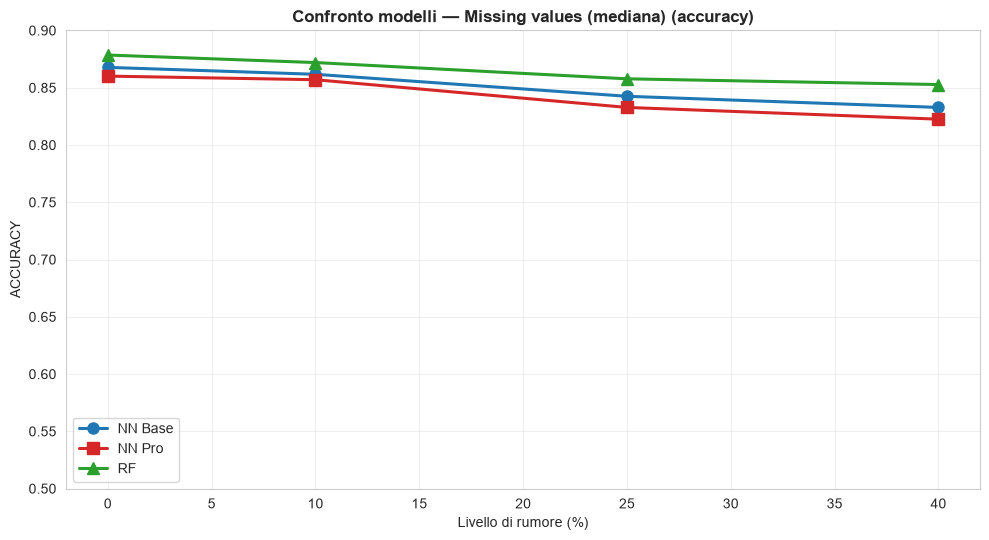
\includegraphics[width=0.86\textwidth]{mv_compare_acc}\\[8pt]
	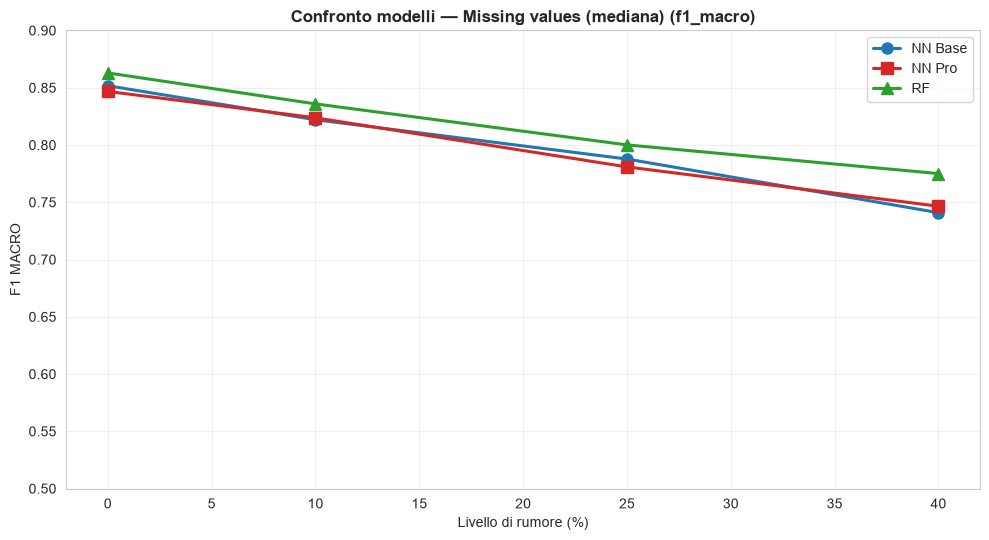
\includegraphics[width=0.86\textwidth]{mv_compare_f1}
	\caption{Missing values con imputazione mediana. Il Random Forest mantiene un vantaggio costante a tutti i livelli.}
	\label{fig:mv_acc}
\end{figure}

Il confronto tra media e mediana (Figura~\ref{fig:mv_strat}) ridimensiona le aspettative sull'asimmetria distributiva: il divario tra le due strategie è marginale e senza una direzione univoca. La mediana porta un lieve vantaggio solo sulla rete Base ai livelli di corruzione più alti; sulla rete Pro è invece la media a risultare leggermente migliore; sul Random Forest le due imputazioni si equivalgono. La mediana viene mantenuta come variante canonica per la sua maggiore robustezza teorica alle code, ma sul piano empirico la scelta tra le due incide poco sui risultati finali. Il Random Forest isola con più flessibilità le istanze falsificate perché i suoi operatori si basano su divisioni del campione, non su pesi distribuiti lungo la rete.

\begin{figure}[H]\centering
	\begin{minipage}{0.32\textwidth}\centering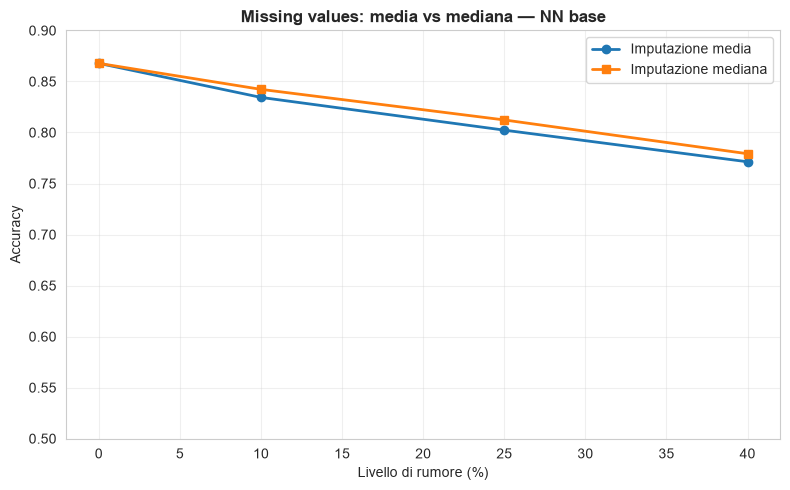
\includegraphics[width=\textwidth]{mv_meanmedian_nnbase}\end{minipage}\hfill
	\begin{minipage}{0.32\textwidth}\centering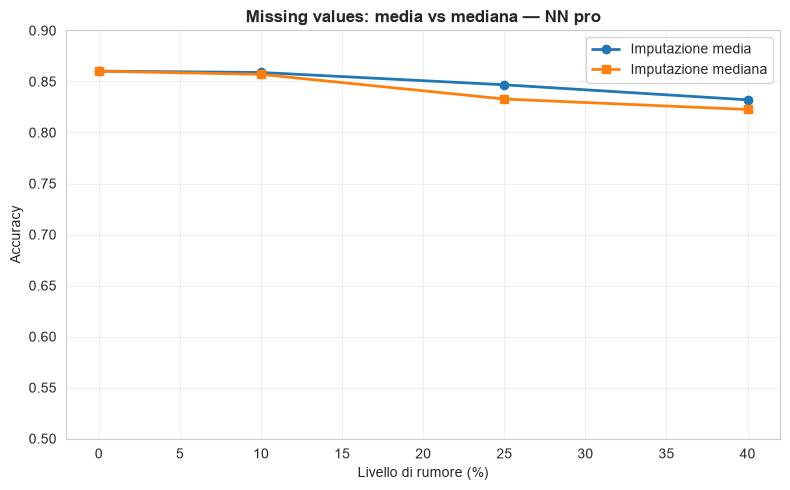
\includegraphics[width=\textwidth]{mv_meanmedian_nnpro}\end{minipage}\hfill
	\begin{minipage}{0.32\textwidth}\centering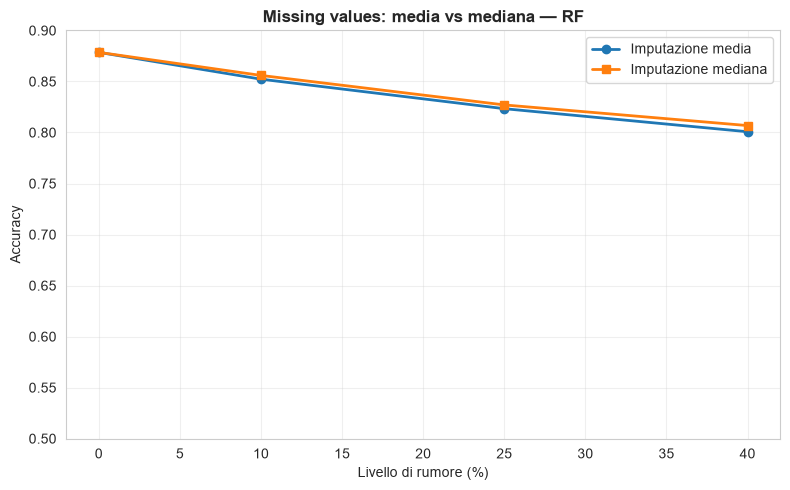
\includegraphics[width=\textwidth]{mv_meanmedian_rf}\end{minipage}
	\caption{Missing values: confronto tra imputazione con media e con mediana per i tre modelli. Le due strategie producono prestazioni pressoché equivalenti; la mediana prevale lievemente solo sulla rete Base ad alta corruzione, mentre sulla rete Pro è la media a risultare marginalmente migliore.}
	\label{fig:mv_strat}
\end{figure}

\begin{figure}[H]\centering
	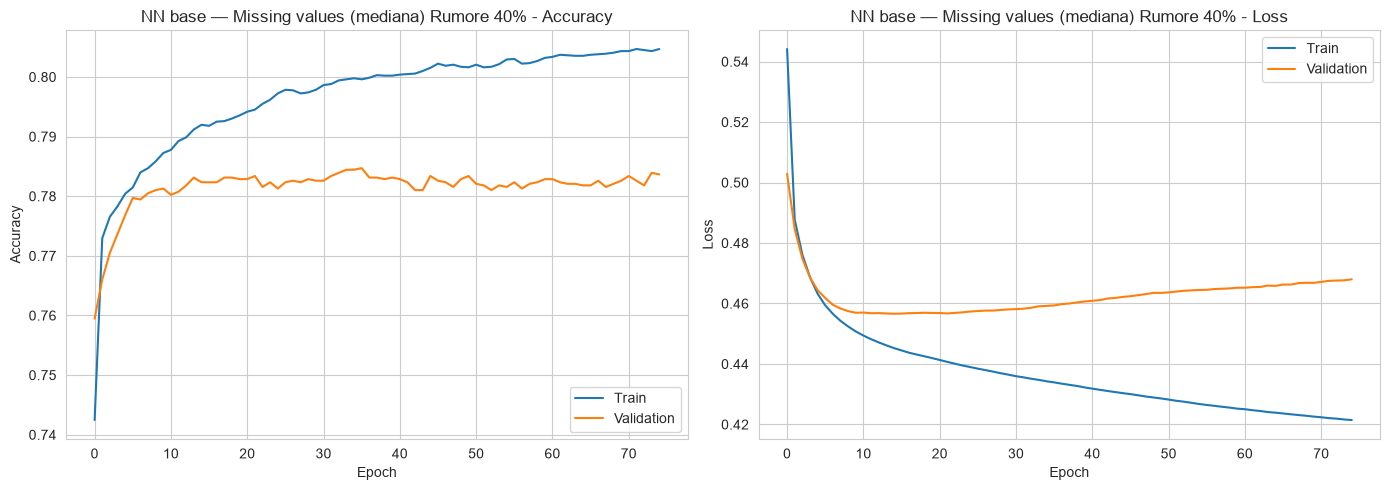
\includegraphics[width=0.9\textwidth]{mv_nnbase_curve40}\\[8pt]
	\begin{minipage}{0.49\textwidth}\centering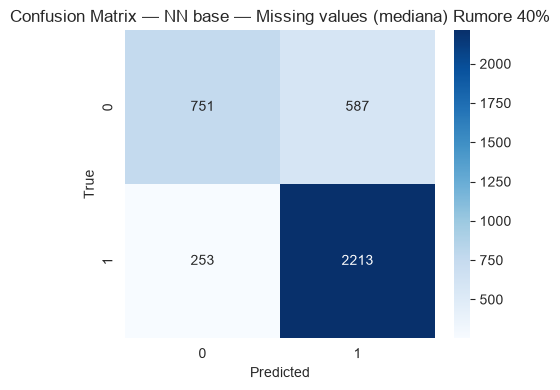
\includegraphics[width=\textwidth]{mv_nnbase_cm40}\end{minipage}\hfill
	\begin{minipage}{0.49\textwidth}\centering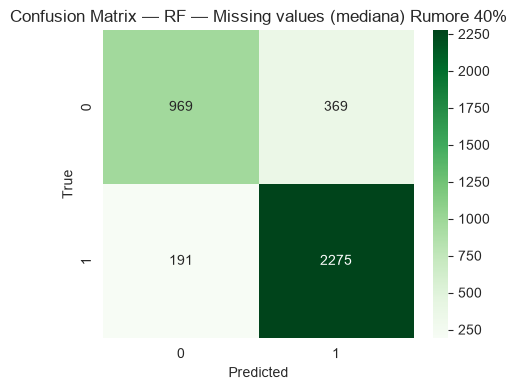
\includegraphics[width=\textwidth]{mv_rf_cm40}\end{minipage}
	\caption{Missing values (mediana) al 40\%: curve della rete Base e matrici di confusione. L'addestramento è regolare; gli errori pesano sugli adroni.}
	\label{fig:mv_cm}
\end{figure}

% ---------- 9.5 Outlier ----------
\subsection{Outlier}

Contrariamente alle aspettative, gli outlier rappresentano il disturbo meno impattante tra quelli analizzati (Tabella~\ref{tab:out}). L'accuratezza resta attorno all'$85\%$--$87\%$, senza tendenze degradative significative (Figura~\ref{fig:out_acc}). La ragione non sta tanto nel trattamento applicato quanto nella natura stessa del disturbo: le righe corrotte assumono valori a $\pm 5$ deviazioni standard con segno casuale, del tutto scorrelato dall'etichetta. Il loro contributo al gradiente si media verso zero e i modelli, valutati su un test set pulito, ne risentono poco.

\begin{table}[H]\centering\footnotesize
\caption{Outlier (winsorizzazione): metriche al variare della frazione di campioni anomali.}\label{tab:out}
\begin{tabular}{c *{9}{c}}
\toprule
 & \multicolumn{3}{c}{NN Base} & \multicolumn{3}{c}{NN Pro} & \multicolumn{3}{c}{Random Forest}\\
\cmidrule(lr){2-4}\cmidrule(lr){5-7}\cmidrule(lr){8-10}
Rumore & Acc & F1$_m$ & AUC & Acc & F1$_m$ & AUC & Acc & F1$_m$ & AUC \\
\midrule
Pulito & 0.8678 & 0.85 & 0.9214 & 0.8601 & 0.85 & 0.9238 & 0.8785 & 0.86 & 0.9300 \\
10\% & 0.8657 & 0.85 & 0.9196 & 0.8583 & 0.84 & 0.9220 & 0.8788 & 0.86 & 0.9295 \\
25\% & 0.8628 & 0.84 & 0.9160 & 0.8441 & 0.83 & 0.9173 & 0.8751 & 0.86 & 0.9267 \\
40\% & 0.8615 & 0.84 & 0.9116 & 0.8541 & 0.84 & 0.9201 & 0.8736 & 0.86 & 0.9250 \\
\bottomrule
\end{tabular}
\end{table}


\begin{figure}[H]\centering
	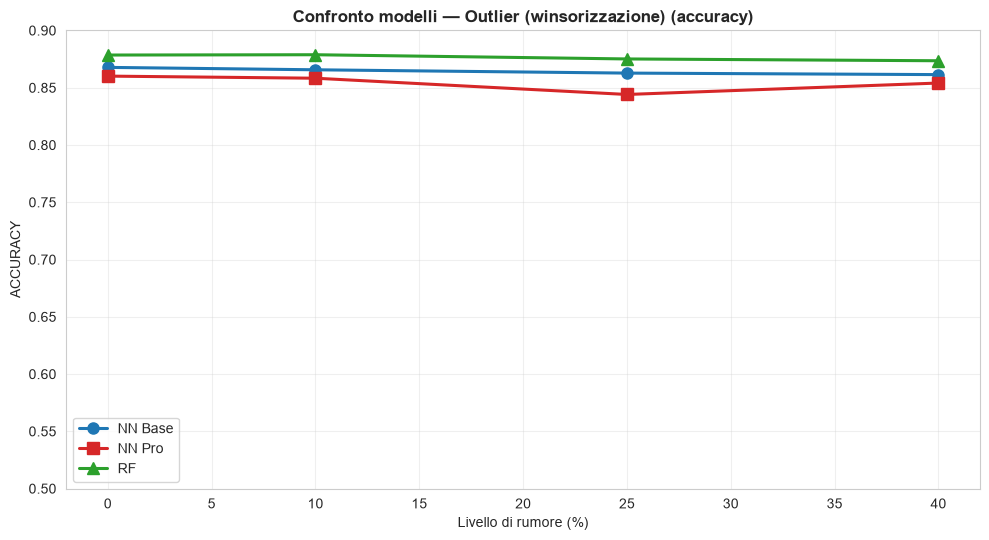
\includegraphics[width=0.86\textwidth]{out_compare_acc}\\[8pt]
	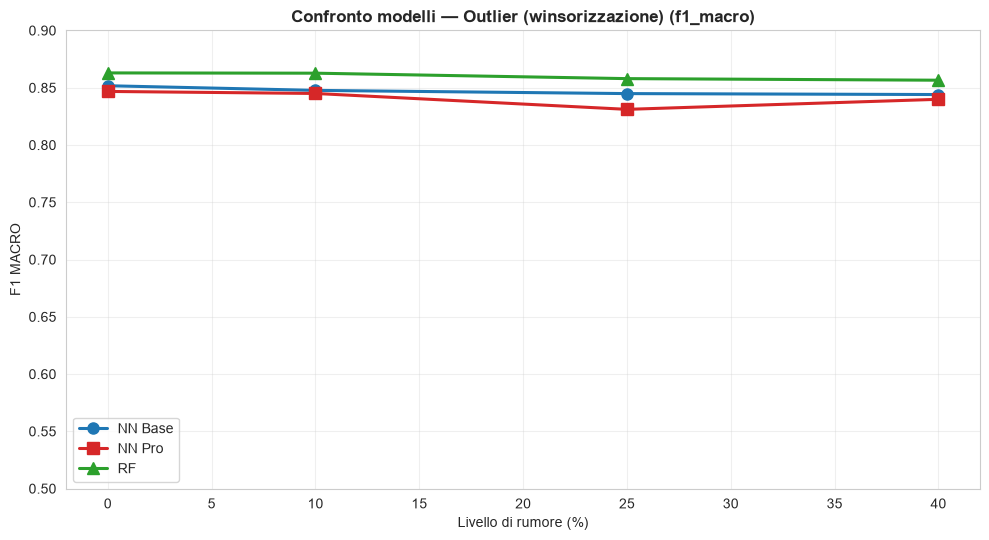
\includegraphics[width=0.86\textwidth]{out_compare_f1}
	\caption{Outlier con winsorizzazione. Curve prestazionali pressoché inalterate.}
	\label{fig:out_acc}
\end{figure}

Le differenze tra le tre strategie di mitigazione (Figura~\ref{fig:out_strat}) rimangono esigue. Lasciare gli outlier invariati, winsorizzare o imputare produce risultati quasi sovrapponibili. Questa equivalenza conferma che a tassi di corruzione elevati la winsorizzazione al $5\%$ è in larga parte inefficace: quando una frazione consistente di valori è collassata su $\pm 5$, i percentili stessi risultano saturi e il troncamento non rimuove gli estremi. La robustezza osservata va quindi attribuita all'intrinseca innocuità del disturbo più che alla strategia di mitigazione. La winsorizzazione viene comunque mantenuta come variante canonica per prudenza, in quanto misura precauzionale senza controindicazioni (Figura~\ref{fig:out_cm}).

\begin{figure}[H]\centering
	\begin{minipage}{0.32\textwidth}\centering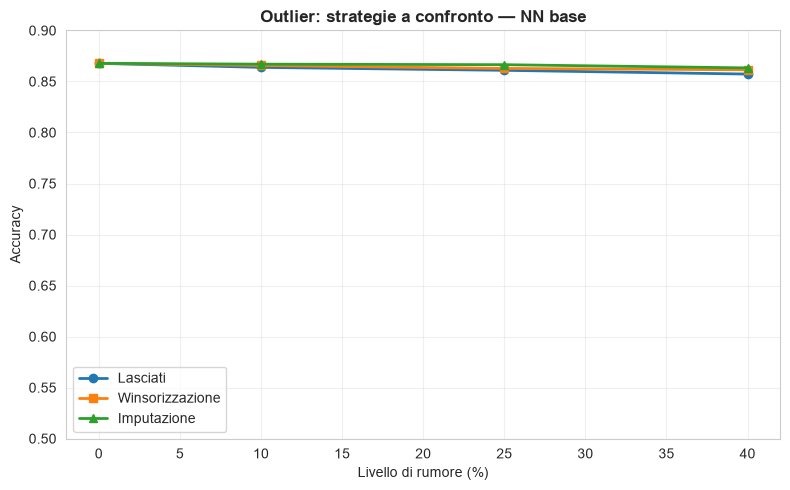
\includegraphics[width=\textwidth]{out_strategies_nnbase}\end{minipage}\hfill
	\begin{minipage}{0.32\textwidth}\centering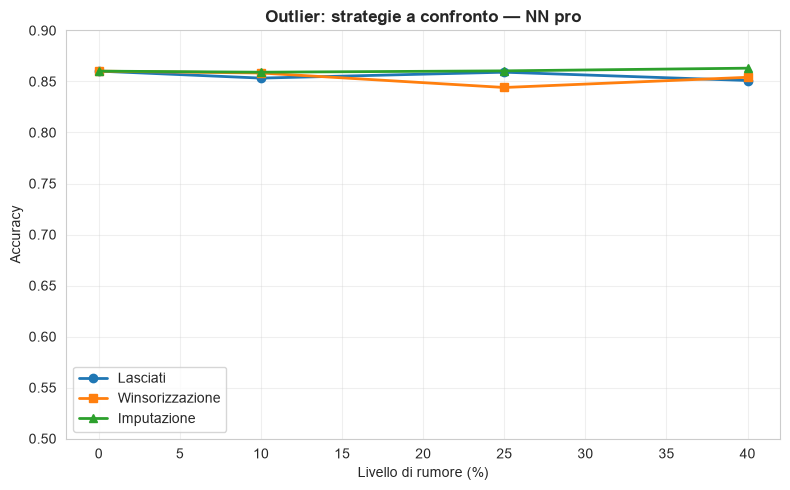
\includegraphics[width=\textwidth]{out_strategies_nnpro}\end{minipage}\hfill
	\begin{minipage}{0.32\textwidth}\centering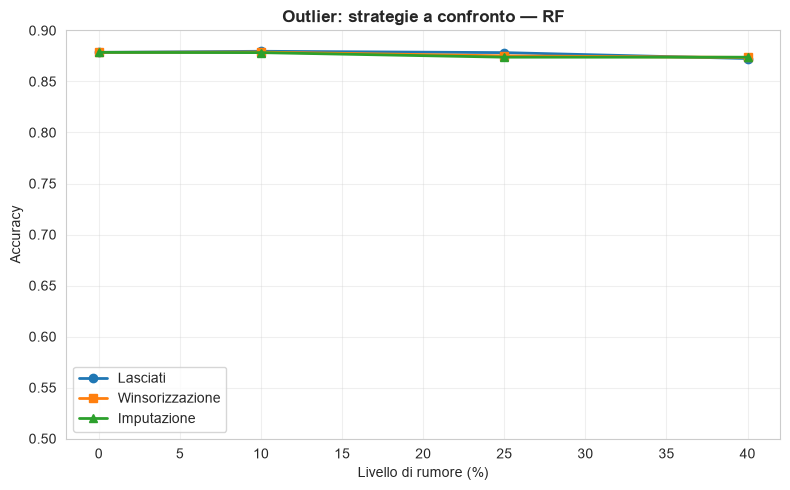
\includegraphics[width=\textwidth]{out_strategies_rf}\end{minipage}
	\caption{Outlier: confronto tra le strategie. Le differenze sono minimali, supportate in buona parte dal preprocessing di standardizzazione.}
	\label{fig:out_strat}
\end{figure}

\begin{figure}[H]\centering
	\begin{minipage}{0.49\textwidth}\centering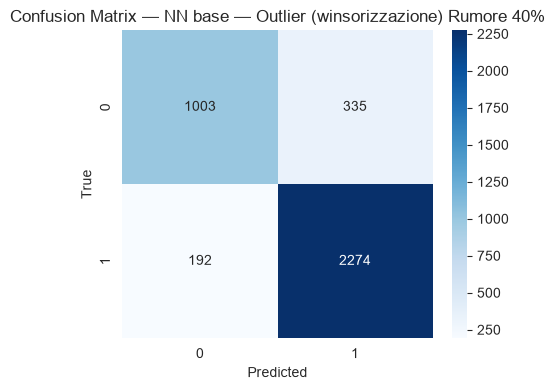
\includegraphics[width=\textwidth]{out_nnbase_cm40}\end{minipage}\hfill
	\begin{minipage}{0.49\textwidth}\centering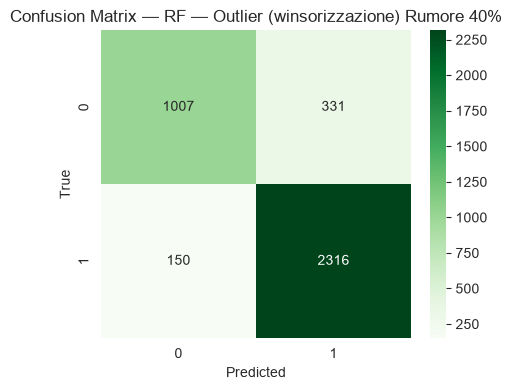
\includegraphics[width=\textwidth]{out_rf_cm40}\end{minipage}
	\caption{Outlier (winsorizzazione) al 40\%: matrici di confusione. Prestazioni indistinguibili dal caso pulito.}
	\label{fig:out_cm}
\end{figure}

% ---------- 9.6 Missing feature ----------
\subsection{Missing feature (sensore guasto)}

La rimozione completa di intere feature produce effetti catastrofici, simili al label noise. Azzerando solo \texttt{fAlpha} (Tabella~\ref{tab:mf}) si registra già una caduta immediata di 4 o 5 punti; arrivando a coprire le cinque feature principali, tutti i modelli testati crollano tra il $70\%$ e il $74\%$ di accuratezza (Figura~\ref{fig:mf_acc}).

\begin{table}[H]\centering\footnotesize
\caption{Missing feature: metriche rimuovendo le feature piu\' importanti (10\%$\to$top-1, 25\%$\to$top-3, 40\%$\to$top-5).}\label{tab:mf}
\begin{tabular}{c *{9}{c}}
\toprule
 & \multicolumn{3}{c}{NN Base} & \multicolumn{3}{c}{NN Pro} & \multicolumn{3}{c}{Random Forest}\\
\cmidrule(lr){2-4}\cmidrule(lr){5-7}\cmidrule(lr){8-10}
Rumore & Acc & F1$_m$ & AUC & Acc & F1$_m$ & AUC & Acc & F1$_m$ & AUC \\
\midrule
Pulito & 0.8678 & 0.85 & 0.9214 & 0.8601 & 0.85 & 0.9238 & 0.8785 & 0.86 & 0.9300 \\
10\% & 0.8215 & 0.79 & 0.8675 & 0.8052 & 0.79 & 0.8716 & 0.8294 & 0.80 & 0.8788 \\
25\% & 0.7773 & 0.74 & 0.8007 & 0.7574 & 0.73 & 0.7991 & 0.7836 & 0.75 & 0.8195 \\
40\% & 0.7303 & 0.67 & 0.7413 & 0.6995 & 0.67 & 0.7347 & 0.7363 & 0.68 & 0.7494 \\
\bottomrule
\end{tabular}
\end{table}


\begin{figure}[H]\centering
	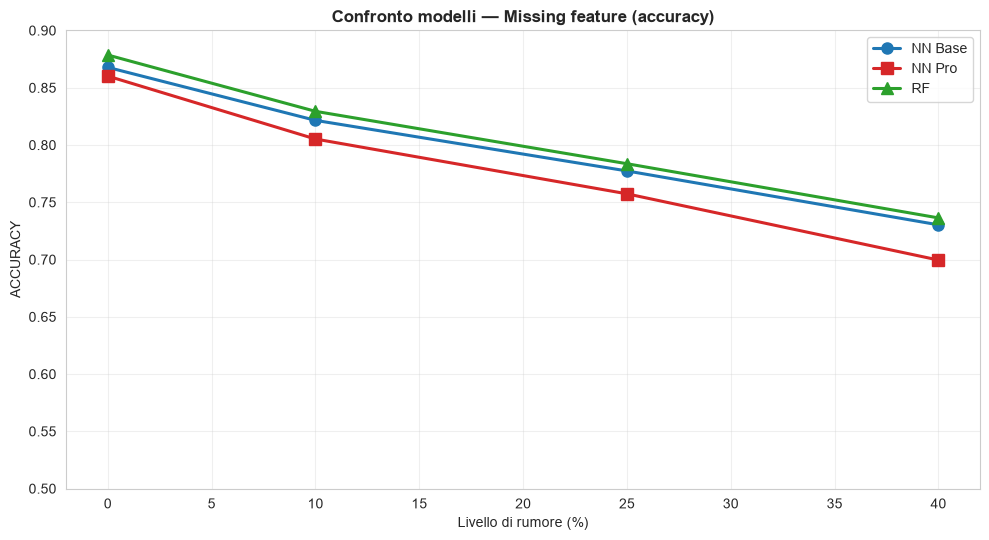
\includegraphics[width=0.86\textwidth]{mf_compare_acc}\\[8pt]
	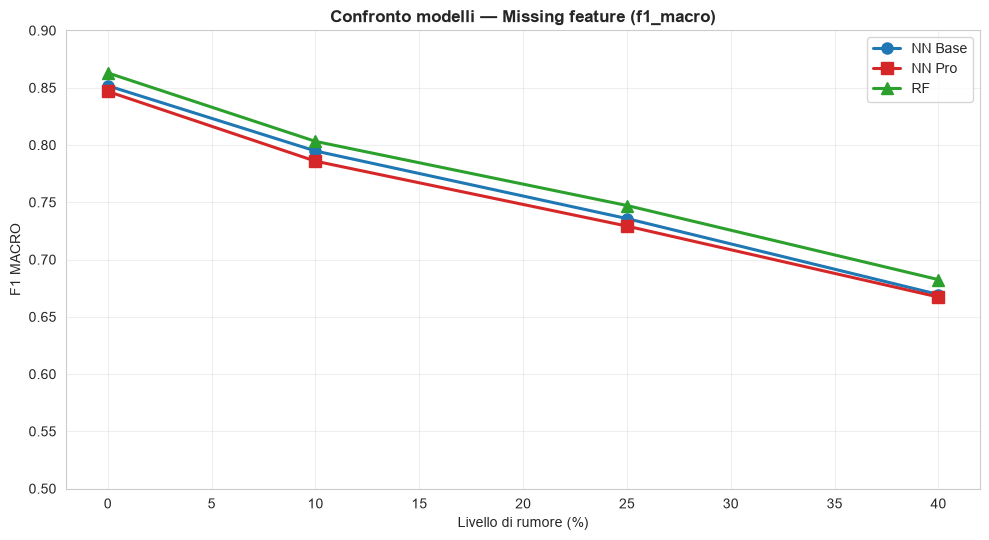
\includegraphics[width=0.86\textwidth]{mf_compare_f1}
	\caption{Missing feature: accuratezza (in alto) e F1 macro (in basso). Rimuovere \texttt{fAlpha} genera il declino più severo registrato fin dalla prima istanza.}
	\label{fig:mf_acc}
\end{figure}

Questo scenario evidenzia l'importanza reale di \texttt{fAlpha}. Essendo quasi scorrelata dalle altre feature, la sua rimozione provoca una perdita insostituibile. In contrasto con il rumore sulle feature, qui la totale assenza di informazione paralizza anche i meccanismi di regolarizzazione, spingendo la rete Pro in fondo alla classifica ($0{,}6995$ al $40\%$). La rigidità dei meccanismi anti-overfitting, che in altri scenari aiutano, qui diventa un limite. La rimozione delle feature danneggia soprattutto la capacità di riconoscere gli adroni, annientando il potere discriminante sulla classe minoritaria (Figure~\ref{fig:mf_cm} e \ref{fig:mf_progress}).

\begin{figure}[H]\centering
	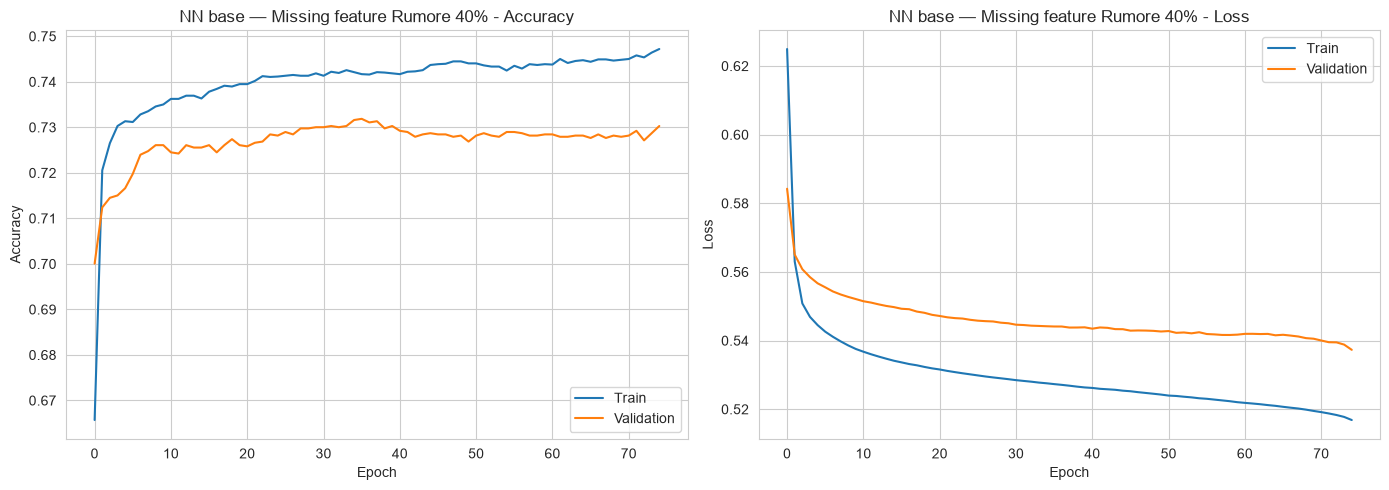
\includegraphics[width=0.9\textwidth]{mf_nnbase_curve40}\\[8pt]
	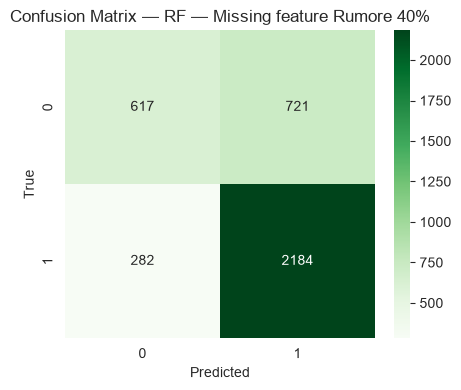
\includegraphics[width=0.5\textwidth]{mf_rf_cm40}
	\caption{Missing feature al 40\%. Senza le feature più informative i modelli perdono potere discriminante intrinseco, pur mantenendo learning curves stabili e vicine.}
	\label{fig:mf_cm}
\end{figure}

\begin{figure}[H]\centering
	\begin{minipage}{0.32\textwidth}\centering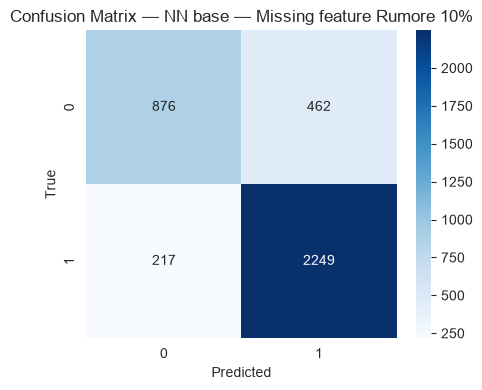
\includegraphics[width=\textwidth]{mf_nnbase_cm10}\end{minipage}\hfill
	\begin{minipage}{0.32\textwidth}\centering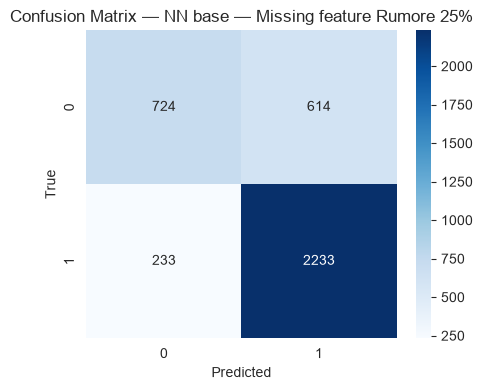
\includegraphics[width=\textwidth]{mf_nnbase_cm25}\end{minipage}\hfill
	\begin{minipage}{0.32\textwidth}\centering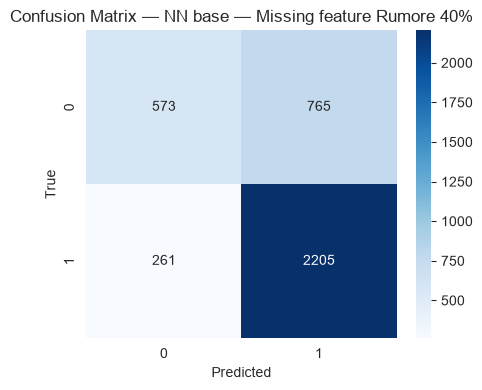
\includegraphics[width=\textwidth]{mf_nnbase_cm40}\end{minipage}
	\caption{Missing feature, rete Base: matrici di confusione. Rimuovendo le feature, la capacità di discriminazione sugli adroni svanisce progressivamente.}
	\label{fig:mf_progress}
\end{figure}

% ============================================================
% 10. SINTESI TRASVERSALE
% ============================================================
\section{Sintesi trasversale}\label{sec:sintesi}

Dopo aver analizzato i singoli scenari, la visione d'insieme (Figura~\ref{fig:aggr}) mostra su un unico asse i livelli di degrado subiti da ciascun modello per ogni tipo di rumore.

\begin{figure}[H]\centering
	\begin{minipage}{0.32\textwidth}\centering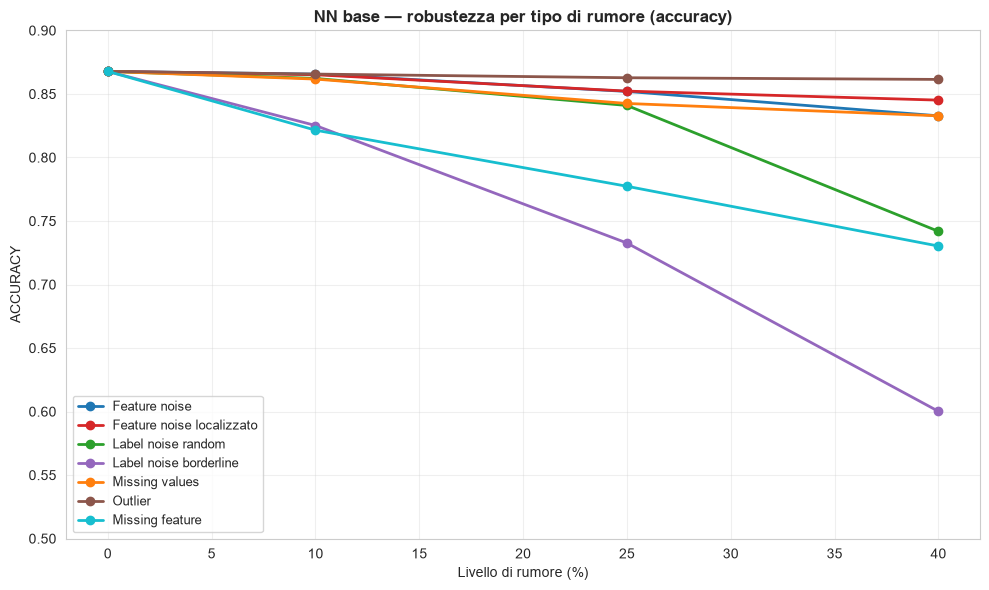
\includegraphics[width=\textwidth]{aggr_nnbase_acc}\end{minipage}\hfill
	\begin{minipage}{0.32\textwidth}\centering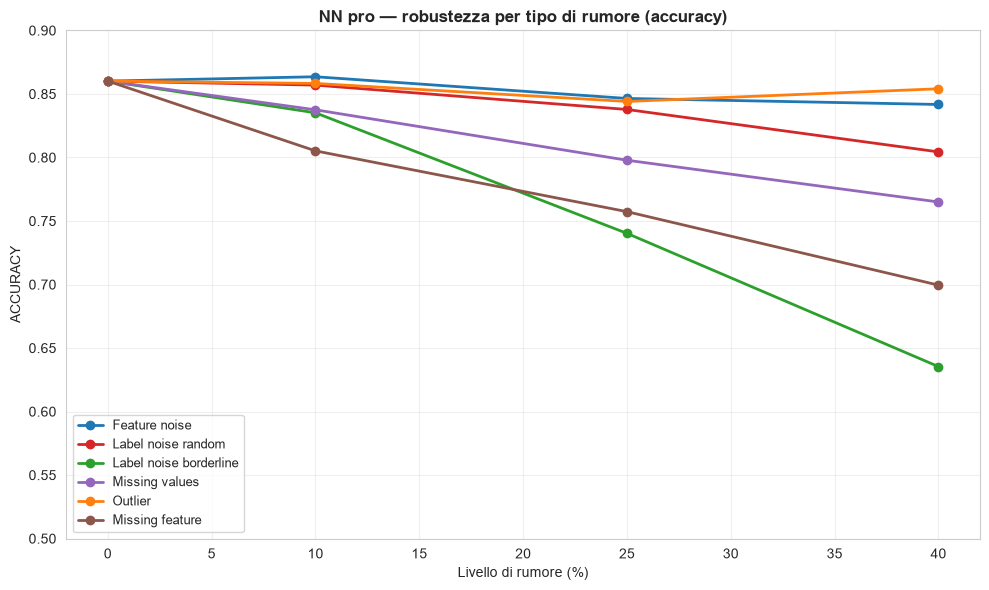
\includegraphics[width=\textwidth]{aggr_nnpro_acc}\end{minipage}\hfill
	\begin{minipage}{0.32\textwidth}\centering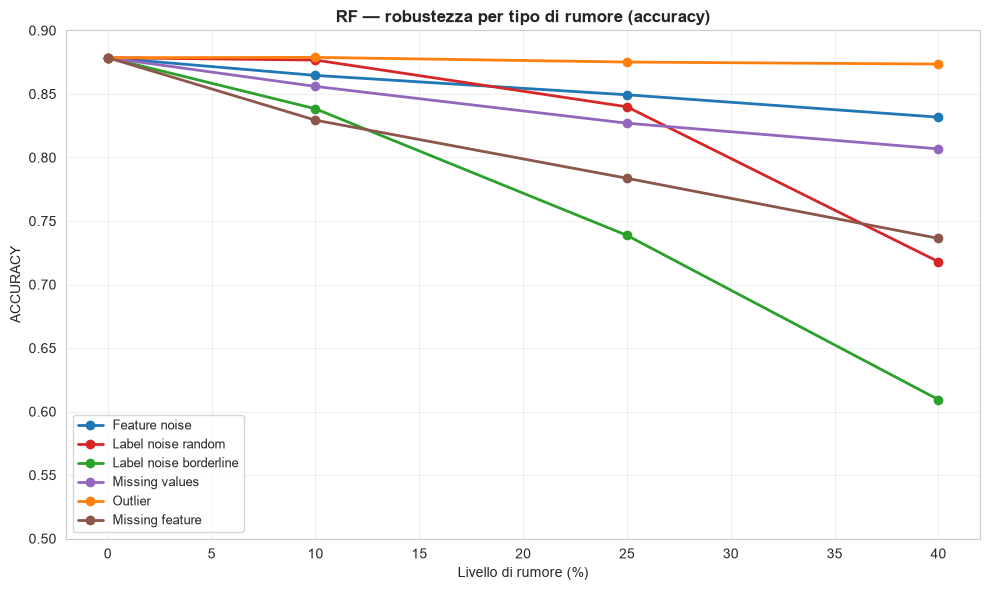
\includegraphics[width=\textwidth]{aggr_rf_acc}\end{minipage}\\[4pt]
	\begin{minipage}{0.32\textwidth}\centering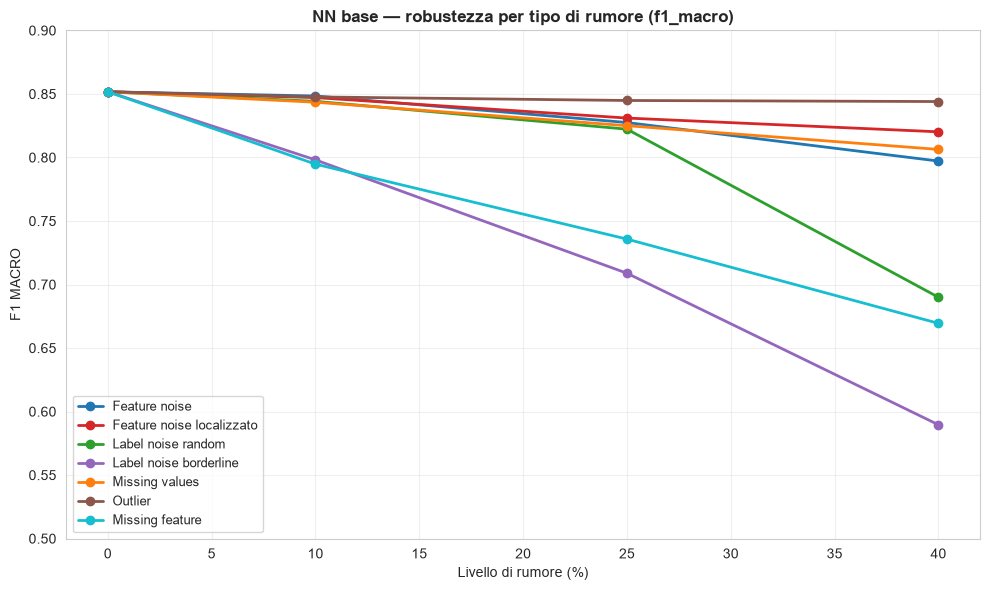
\includegraphics[width=\textwidth]{aggr_nnbase_f1}\end{minipage}\hfill
	\begin{minipage}{0.32\textwidth}\centering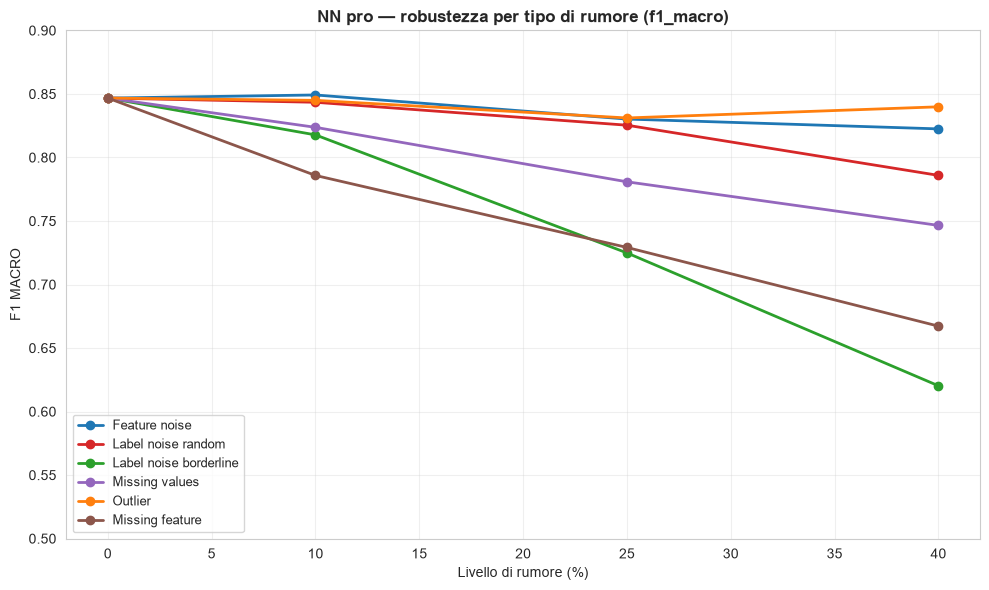
\includegraphics[width=\textwidth]{aggr_nnpro_f1}\end{minipage}\hfill
	\begin{minipage}{0.32\textwidth}\centering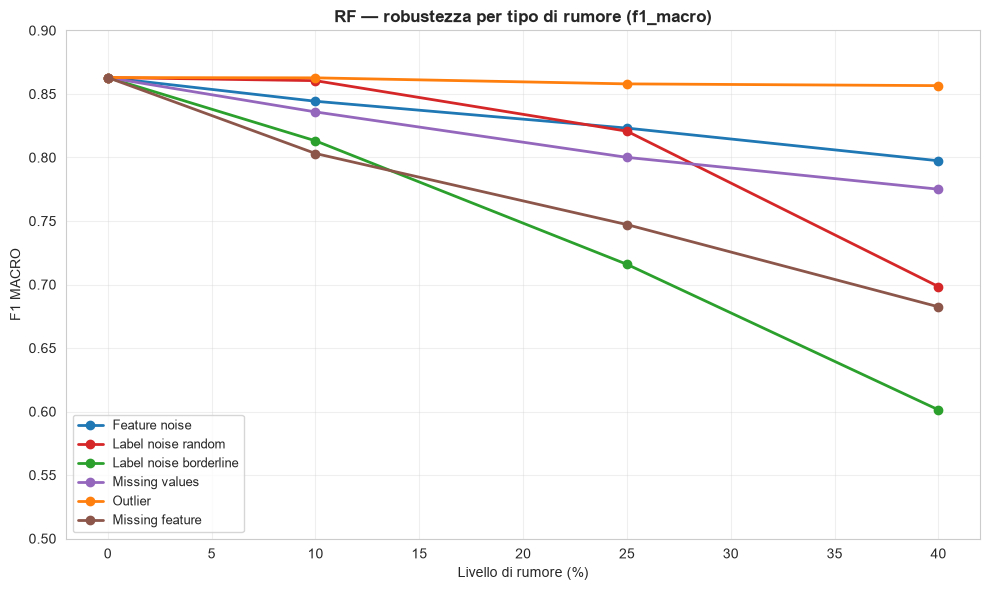
\includegraphics[width=\textwidth]{aggr_rf_f1}\end{minipage}
	\caption{Robustezza per tipo di rumore. Emerge costantemente l'outlier come disturbo innocuo e il label noise borderline come criticità massima.}
	\label{fig:aggr}
\end{figure}

I risultati delineano una gerarchia di vulnerabilità condivisa tra tutti i modelli. Gli outlier sono i meno dannosi, seguiti da feature noise e valori mancanti, che producono cali moderati e gestibili. All'estremo opposto, il label noise borderline è la perturbazione più severa, portando tutti i modelli al collasso. La heatmap (Figura~\ref{fig:heatmap}) cristallizza questi trend nel caso peggiore al $40\%$ di corruzione, mostrando cromaticamente l'annullamento delle prestazioni con il label noise borderline rispetto alla quasi-invarianza con gli outlier.

\begin{figure}[H]\centering
	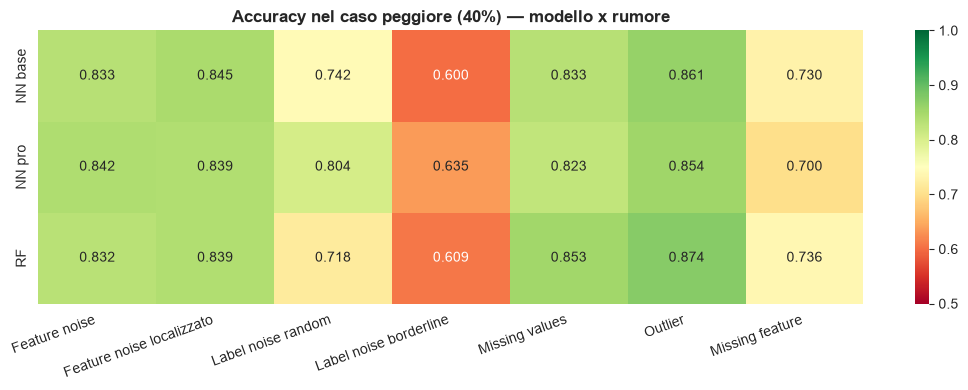
\includegraphics[width=0.98\textwidth]{summary_heatmap}
	\caption{Accuratezza nel caso peggiore (40\%) per ogni combinazione. Il rosso intenso sul label noise borderline indica il collasso predittivo.}
	\label{fig:heatmap}
\end{figure}

Sul fronte della tenuta (Figura~\ref{fig:degr}), la rete Pro mostra la maggiore tolleranza ai disturbi continui sulle feature, ma soffre di più quando una feature viene completamente rimossa. In quello scenario, il Random Forest domina per flessibilità strutturale.

\begin{figure}[H]\centering
	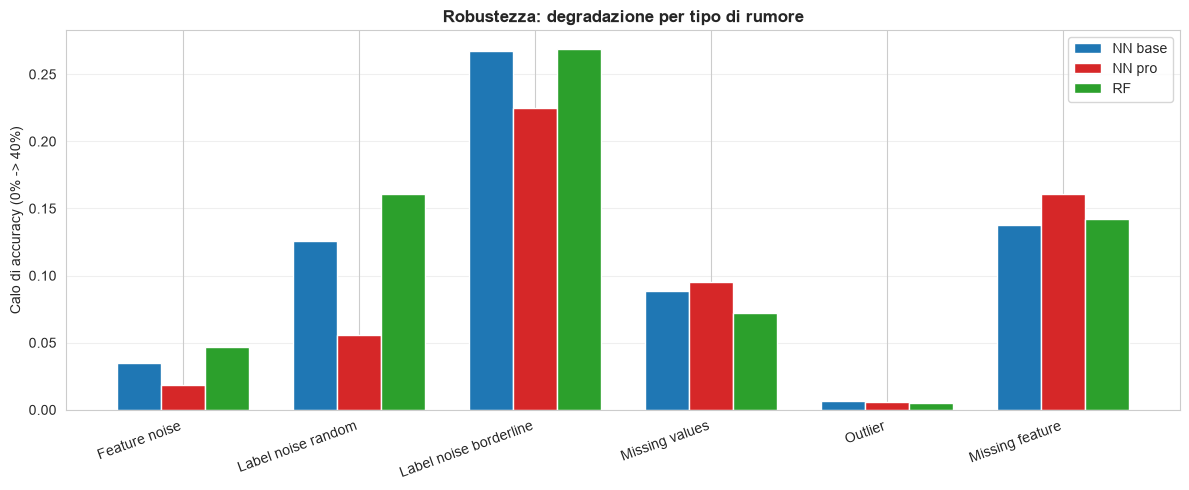
\includegraphics[width=0.98\textwidth]{summary_degradation}
	\caption{Calo di accuratezza. Barre contenute indicano maggiore tenuta ai gradienti spuri e al data leakage.}
	\label{fig:degr}
\end{figure}

Mediando su tutti i tipi di rumore (Figura~\ref{fig:rank}), le distanze globali si assottigliano fino quasi alla sovrapposizione. La rete Pro si posiziona in testa ($0{,}785$), seguita dal Random Forest ($0{,}780$) e dalla rete Base ($0{,}778$). Le distanze sono però talmente ridotte che la scelta del modello non può basarsi su questo numero medio: dipende dal tipo di errore atteso nel dominio applicativo reale.

\begin{figure}[H]\centering
	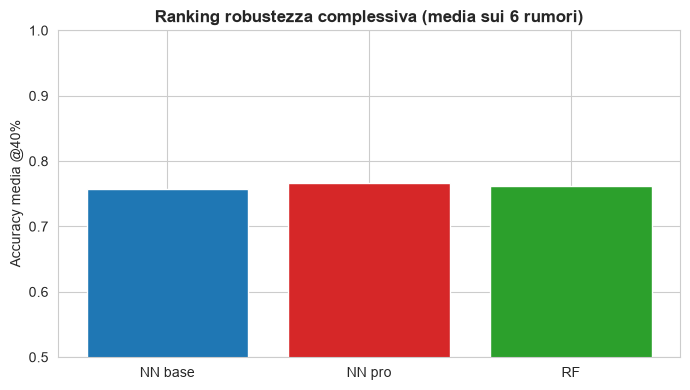
\includegraphics[width=0.74\textwidth]{summary_ranking}
	\caption{Robustezza complessiva (accuratezza media). I tre modelli convergono in uno spazio di deviazione trascurabile.}
	\label{fig:rank}
\end{figure}

Le curve ROC incrociate sul feature noise gaussiano (Figura~\ref{fig:roc}) confermano che il rumore erode solo limitatamente la capacità di ranking dei modelli, con la rete Pro che si posiziona in modo coerente rispetto alla rete Base anche in presenza di disturbo.

\begin{figure}[H]\centering
	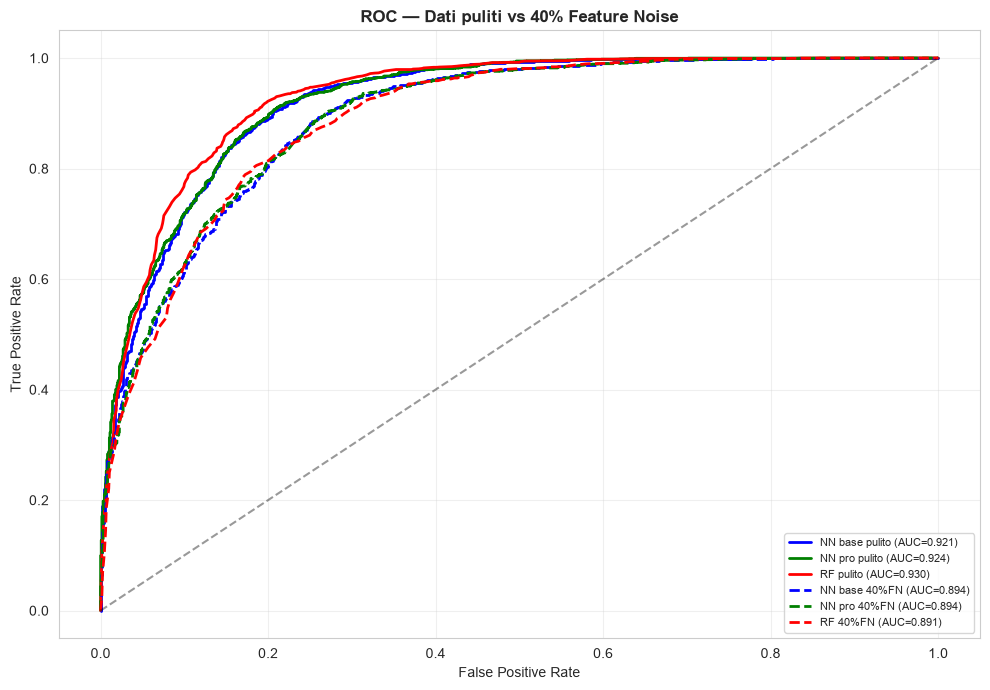
\includegraphics[width=0.90\textwidth]{roc_clean_vs_fn40}
	\caption{Curve ROC dei tre modelli su dati puliti (continue) e con 40\% di feature noise (tratteggiate). Il feature noise erode limitatamente la classificazione ordinale.}
	\label{fig:roc}
\end{figure}

\subsection{Controllo multi-seed}\label{sec:multiseed}

Tutti i risultati discussi finora derivano da un singolo seme casuale (\texttt{seed = 42}). Per escludere che il degrado osservato dipenda da una partizione dei dati o da un'inizializzazione dei pesi particolarmente favorevole o sfavorevole, l'esperimento di feature noise è stato ripetuto identicamente su cinque semi distinti: $\{42, 7, 123, 2024, 99\}$. Ogni seme governa contemporaneamente il rumore gaussiano, lo split train/validation/test e l'inizializzazione dei tre modelli. Per ciascun livello di corruzione si riportano media e deviazione standard delle metriche (Tabella~\ref{tab:multiseed}).

\begin{table}[H]\centering\footnotesize
\caption{Controllo multi-seed sul feature noise: media $\pm$ deviazione standard delle metriche sui cinque semi $\{42, 7, 123, 2024, 99\}$. Le deviazioni standard restano dell'ordine del millesimo, ampiamente inferiori al divario tra livelli di rumore.}\label{tab:multiseed}
\begin{tabular}{ll ccc}
\toprule
Modello & Rumore & Accuracy & F1$_m$ & AUC \\
\midrule
NN Base & Pulito & $0.8685 \pm 0.0027$ & $0.8514 \pm 0.0029$ & $0.9220 \pm 0.0015$ \\
        & 10\%   & $0.8672 \pm 0.0018$ & $0.8487 \pm 0.0025$ & $0.9198 \pm 0.0014$ \\
        & 25\%   & $0.8526 \pm 0.0020$ & $0.8270 \pm 0.0024$ & $0.9068 \pm 0.0016$ \\
        & 40\%   & $0.8342 \pm 0.0031$ & $0.7997 \pm 0.0040$ & $0.8924 \pm 0.0027$ \\
\midrule
NN Pro  & Pulito & $0.8638 \pm 0.0035$ & $0.8497 \pm 0.0032$ & $0.9241 \pm 0.0010$ \\
        & 10\%   & $0.8631 \pm 0.0036$ & $0.8479 \pm 0.0030$ & $0.9204 \pm 0.0012$ \\
        & 25\%   & $0.8464 \pm 0.0045$ & $0.8293 \pm 0.0036$ & $0.9056 \pm 0.0016$ \\
        & 40\%   & $0.8328 \pm 0.0068$ & $0.8130 \pm 0.0070$ & $0.8924 \pm 0.0012$ \\
\midrule
Random Forest & Pulito & $0.8800 \pm 0.0013$ & $0.8645 \pm 0.0014$ & $0.9308 \pm 0.0009$ \\
        & 10\%   & $0.8646 \pm 0.0024$ & $0.8442 \pm 0.0026$ & $0.9198 \pm 0.0015$ \\
        & 25\%   & $0.8492 \pm 0.0016$ & $0.8228 \pm 0.0016$ & $0.9042 \pm 0.0018$ \\
        & 40\%   & $0.8285 \pm 0.0037$ & $0.7934 \pm 0.0055$ & $0.8881 \pm 0.0028$ \\
\bottomrule
\end{tabular}
\end{table}


L'esito è netto: le deviazioni standard restano nell'ordine del millesimo per ogni combinazione modello--livello, con un valore massimo di appena $0{,}0068$ (rete Pro al $40\%$). Questa dispersione è di un ordine di grandezza inferiore al calo prodotto dal rumore: la sola rete Base perde circa $3{,}4$ punti percentuali di accuratezza passando dai dati puliti al $40\%$. Il degrado è quindi un segnale reale indotto dai dati, non semplice varianza procedurale. Le barre d'errore nelle Figure~\ref{fig:ms_acc} e \ref{fig:ms_f1} sono appena percettibili attorno ai marcatori, a conferma visiva di questa stabilità.

\begin{figure}[H]\centering
	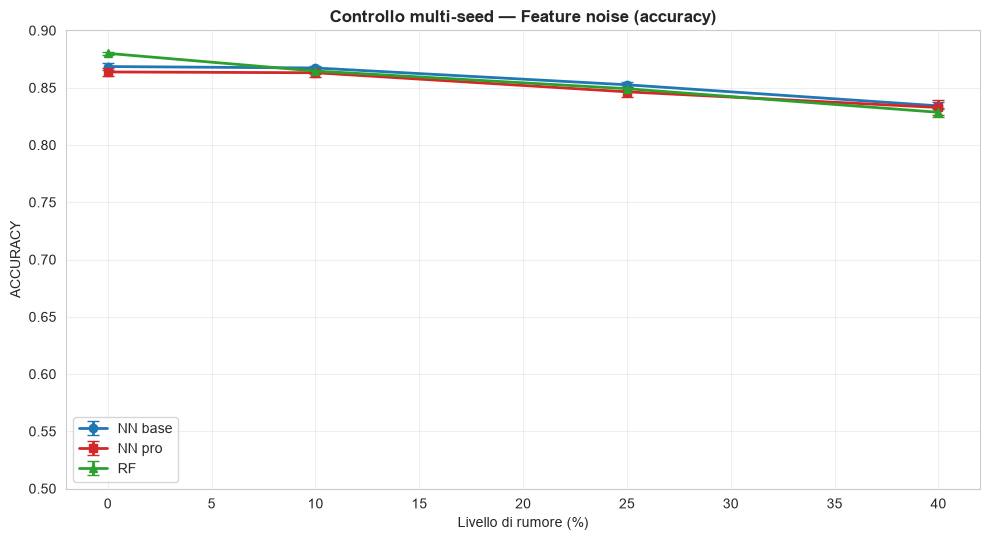
\includegraphics[width=0.82\textwidth]{ms_acc}
	\caption{Controllo multi-seed (feature noise): accuratezza media sui cinque semi al variare del livello di rumore. Le barre d'errore ($\pm 1$ deviazione standard) sono quasi impercettibili, a conferma della riproducibilità del trend.}
	\label{fig:ms_acc}
\end{figure}

\begin{figure}[H]\centering
	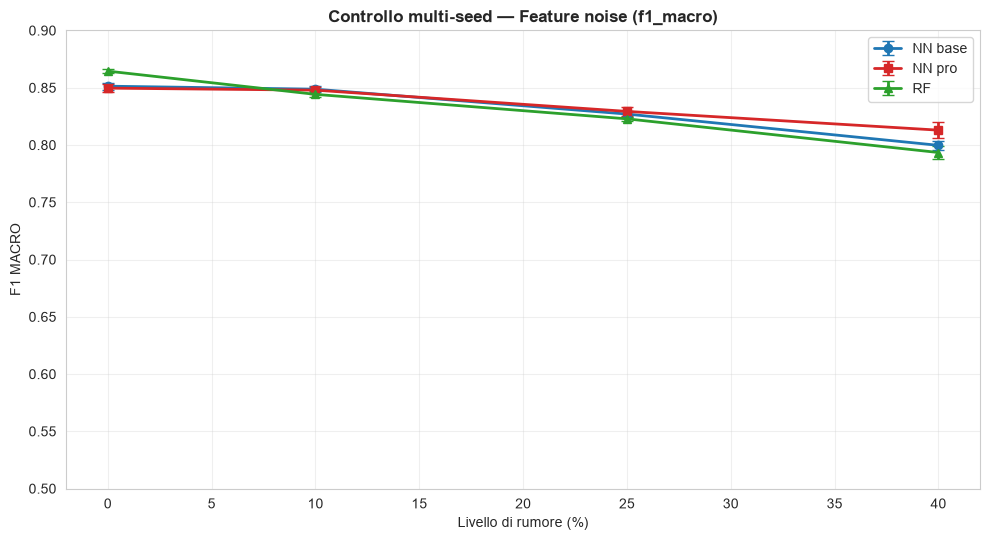
\includegraphics[width=0.82\textwidth]{ms_f1}
	\caption{Controllo multi-seed (feature noise): F1 macro media sui cinque semi. Anche sulla metrica bilanciata l'ordinamento dei modelli e l'entità del degrado restano stabili tra i semi.}
	\label{fig:ms_f1}
\end{figure}

La verifica conferma anche la gerarchia di robustezza emersa con il seme singolo. Il Random Forest parte dal livello più alto sui dati puliti ($0{,}8800$) ma cede terreno più rapidamente, allineandosi alle reti neurali al $40\%$. La rete Pro mostra il degrado più graduale grazie alla regolarizzazione, pur partendo da una base leggermente inferiore. Queste differenze, coerenti tra i cinque semi, escludono che l'ordinamento osservato dipenda da fluttuazioni casuali.

% ============================================================
% 11. PARTE NON SUPERVISIONATA
% ============================================================
\section{Analisi non supervisionata (K-Means)}\label{sec:kmeans}

L'analisi include anche un esperimento di clustering non supervisionato. Il numero di cluster è stato fissato a due, sulla base dell'andamento dell'inerzia (metodo del gomito) e del valore della silhouette, che risulta massimo proprio in corrispondenza di $k=2$ (Figura~\ref{fig:kmeans_k}). Va notato che la silhouette tende strutturalmente a premiare valori di $k$ bassi, quindi costituisce un indizio più che una prova definitiva. Il risultato rispecchia comunque quanto emerso dai modelli supervisionati. Il label noise è del tutto ininfluente sull'orientamento dei centroidi, perché il clustering si basa esclusivamente sulla distanza euclidea, senza accedere alle etichette.

\begin{figure}[H]\centering
	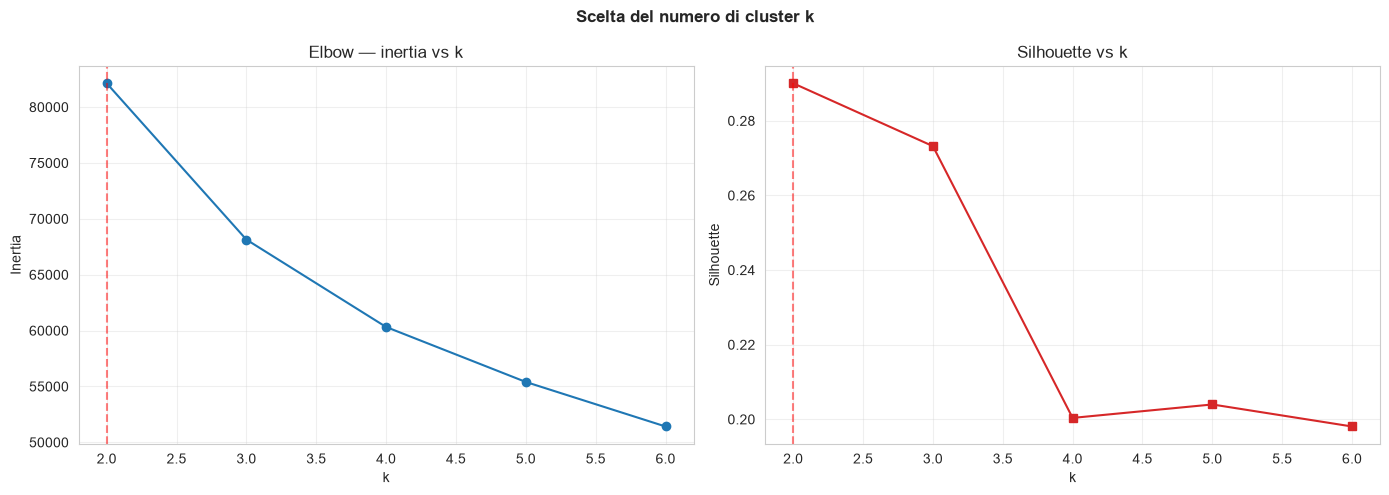
\includegraphics[width=0.92\textwidth]{kmeans_kselection}
	\caption{Scelta del numero di cluster. Inerzia e silhouette indicano in $k=2$ la configurazione spaziale ottimale per la densità esplorata.}
	\label{fig:kmeans_k}
\end{figure}

Le distanze geometriche non riescono però a mappare le differenze fisiche tra gamma e adroni. L'assegnazione spaziale produce un Adjusted Rand Index di 0,006 (quasi nullo) e un indice di purezza paragonabile allo squilibrio probabilistico nativo dei dati. In sintesi, l'algoritmo separa masse numeriche senza alcun legame con la classificazione fisica (Figura~\ref{fig:kmeans}). Le proprietà che distinguono gamma e adroni attraversano i cluster senza offrire separazioni lineari nello spazio delle feature.

\begin{figure}[H]\centering
	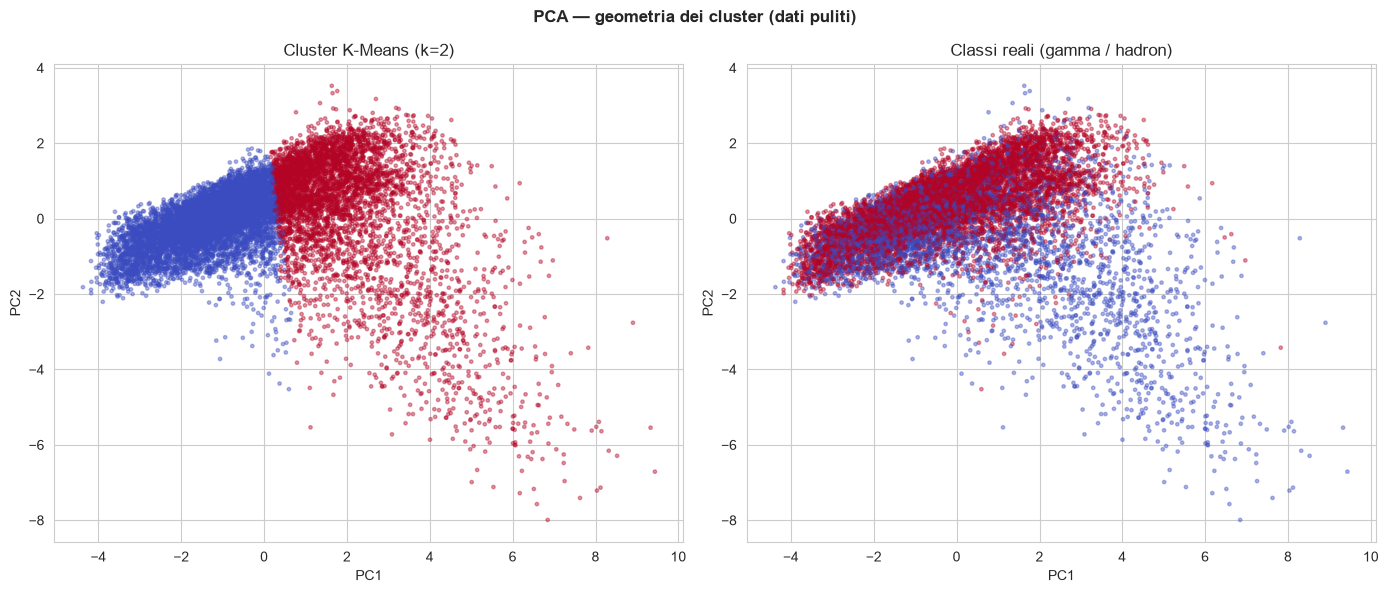
\includegraphics[width=0.98\textwidth]{kmeans_pca}
	\caption{Proiezione PCA: i cluster geometrici non si allineano con la natura fisica e asimmetrica delle collisioni (ARI $\approx 0$).}
	\label{fig:kmeans}
\end{figure}

Introducendo crescente rumore sulle feature (Figure~\ref{fig:kmeans_noise} e \ref{fig:kmeans_noise_pca}), la qualità del clustering peggiora proporzionalmente. Il label noise passa invece invisibile, perché i centroidi non dipendono dalle etichette. Le perturbazioni sulle feature espandono caotica\-mente le nuvole di punti proiettate: le sagome dei cluster si dissolvono in transizioni piatte e la silhouette scende oltre lo $0{,}10$. La vulnerabilità a un tipo di rumore dipende quindi strettamente da quali informazioni il modello utilizza.

\begin{figure}[H]\centering
	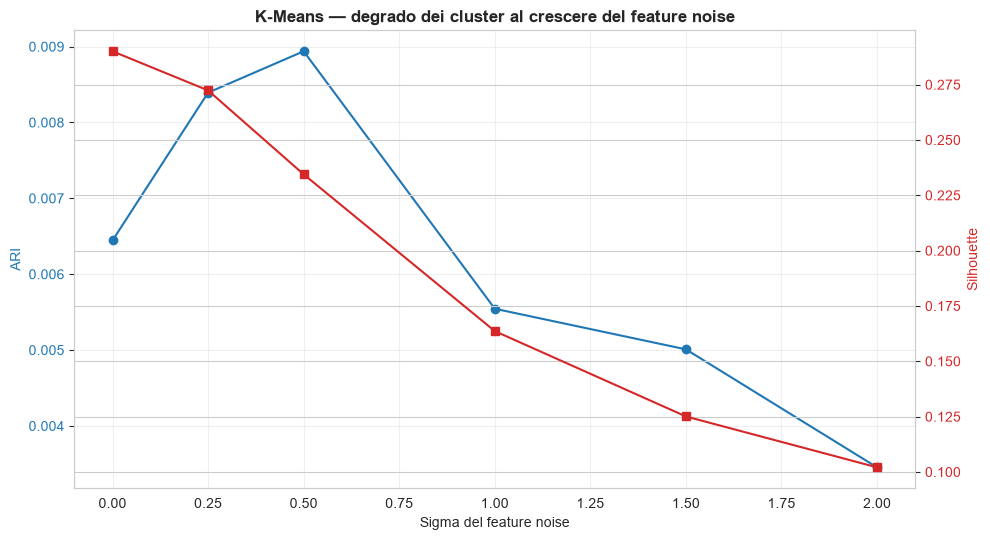
\includegraphics[width=0.86\textwidth]{kmeans_noise}
	\caption{K-Means sotto feature noise: ARI e silhouette dei cluster. La silhouette cala, mentre l'ARI resta vicino a zero.}
	\label{fig:kmeans_noise}
\end{figure}

\begin{figure}[H]\centering
	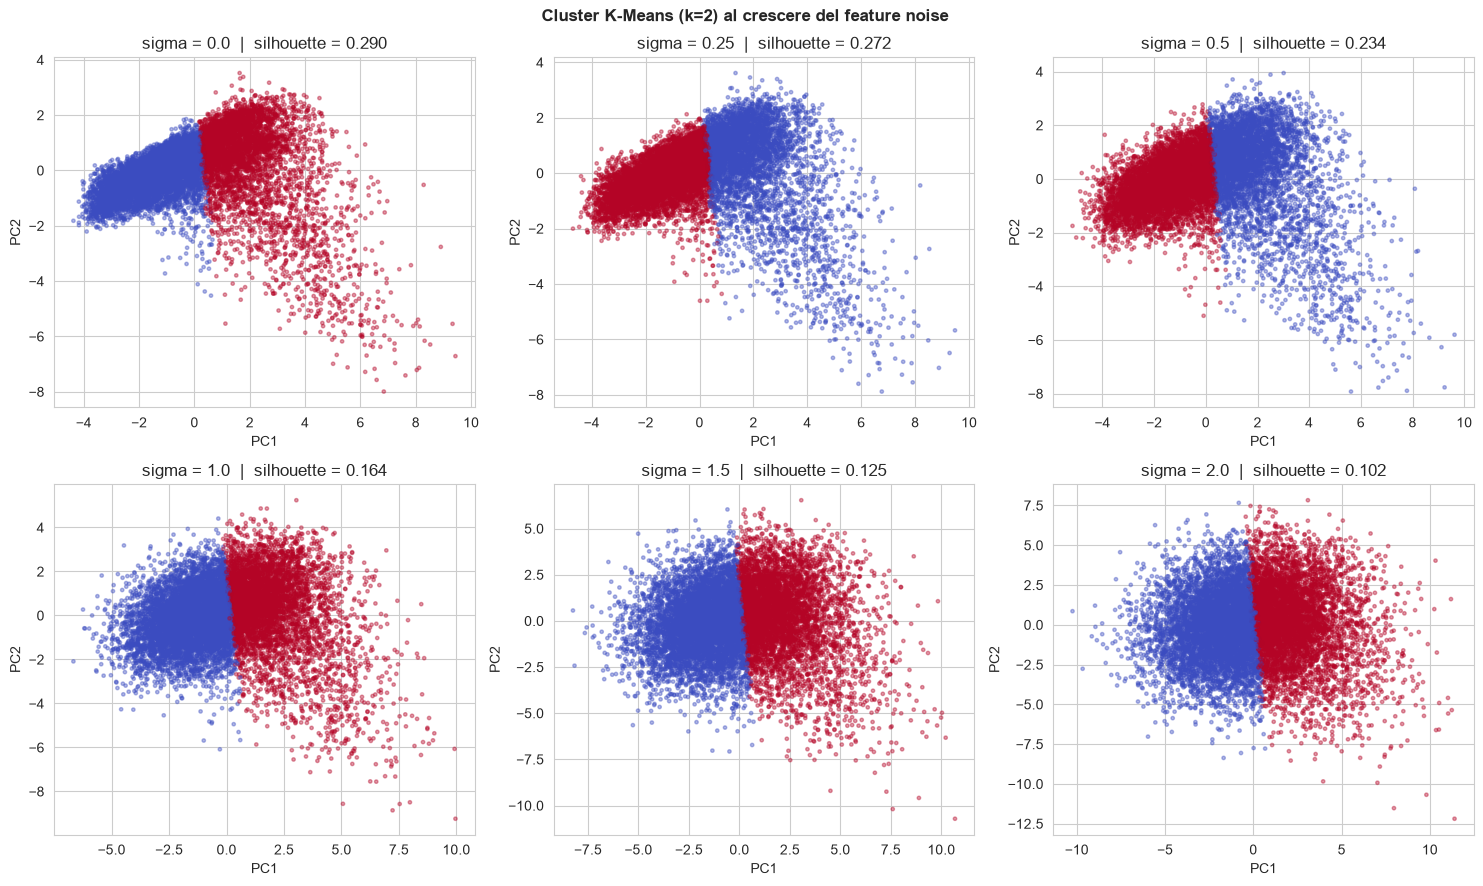
\includegraphics[width=0.92\textwidth]{kmeans_noise_pca}
	\caption{Cluster K-Means (k=2) proiettati sulle prime due componenti (PCA). Al crescere del rumore ($\sigma$) la densità spaziale viene a mancare e le istanze sfumano i propri confini.}
	\label{fig:kmeans_noise_pca}
\end{figure}

% ============================================================
% 12. CONCLUSIONI
% ============================================================
\section{Conclusioni}\label{sec:conclusioni}

Questo studio sposta l'attenzione dalla ricerca del modello migliore in assoluto alla valutazione di quale algoritmo resiste meglio a specifiche tipologie di corruzione dei dati. I risultati delineano un quadro coerente in cui nessuna soluzione è priva di compromessi.

Tra i disturbi analizzati emerge una gerarchia di pericolosità chiara. Gli outlier sono i meno dannosi, con un impatto quasi trascurabile anche senza trattamenti specifici. Feature noise e valori mancanti generano un calo moderato e gestibile, mitigato rispettivamente dalla ridondanza informativa tra le feature e dalle strategie di imputazione. Al contrario, la rimozione delle feature e il label noise sono le anomalie più critiche, per ragioni opposte. Rimuovere una feature elimina informazione predittiva insostituibile: azzerare solo \texttt{fAlpha} risulta più impattante del livello massimo di feature noise. Il label noise, invece, forza i modelli a memorizzare pattern errati. Il caso più estremo è il label noise borderline, che corrompendo le istanze vicine al confine decisionale riduce le prestazioni fino ai livelli di un classificatore banale.

Confrontando i modelli, nessuno prevale in ogni scenario. La rete Pro dimostra l'efficacia della regolarizzazione: l'early stopping la rende particolarmente resistente al label noise random, bloccando la memorizzazione del rumore che penalizza la rete Base. Tuttavia questa stessa propensione a non adattarsi troppo ai dati la penalizza quando una feature viene rimossa del tutto. Il Random Forest si conferma il più solido su dati puliti, valori mancanti e outlier, ma mostra una fragilità notevole di fronte all'inversione casuale delle etichette. La rete Base, pur competitiva su dati puliti, è la più esposta all'aumentare del rumore. La scelta del modello non può prescindere da un'analisi preventiva sui tipi di errore attesi nel dominio applicativo.

L'analisi per classe aggiunge un'ulteriore chiave di lettura. Sotto la maggior parte dei disturbi, il degrado colpisce quasi esclusivamente la classe minoritaria (adroni), mentre il segnale (gamma) continua a essere identificato correttamente. Usare solo l'accuratezza globale avrebbe nascosto questa dinamica. I class weight nella rete Pro si rivelano fondamentali per preservare la capacità di riconoscere la classe rara. Fa eccezione il label noise borderline, che degrada le metriche in modo uniforme su entrambe le classi perché distorce direttamente il confine spaziale.

L'evidenza più significativa riguarda però l'importanza del preprocessing rispetto alla complessità algoritmica. Strategie mirate come l'imputazione dei valori mancanti, la winsorizzazione degli outlier e l'interruzione dell'addestramento basata sulla validation loss permettono di arginare gran parte del degrado. Nessun modello, per quanto sofisticato, può recuperare un'informazione cancellata o falsificata nei punti più sensibili. La robustezza di un sistema predittivo si costruisce prima di tutto nella cura del dato, tanto quanto nella scelta dell'algoritmo. L'esperimento non supervisionato lo conferma: ciò che è critico per un task supervisionato può essere del tutto ininfluente per un approccio basato sulla distanza spaziale.

\end{document}
